% !TEX TS-program = pdflatex
\documentclass{article}   	% use "amsart" instead of "article" for AMSLaTeX format
\usepackage{geometry}                		% See geom\dagetry.pdf to learn the layout options. There are lots.
\geometry{a4paper}                   		% ... or a4paper or a5paper or ... 
%\geometry{landscape}                		% Activate for for rotated page geometry
%\usepackage[parfill]{parskip}    		% Activate to begin paragraphs with an empty line rather than an indent
\usepackage{graphicx}				% Use pdf, png, jpg, or eps§ with pdflatex; use eps in DVI mode
\usepackage{array}							% TeX will automatically convert eps --> pdf in pdflatex		
\usepackage{amssymb,amsmath}
\usepackage{cite}
\usepackage[final]{fixme}
\usepackage{pdfpages}
\usepackage{tabularx}
\usepackage{fancyheadings}
\usepackage{lastpage}
\usepackage{tikz}
\usetikzlibrary{shapes,arrows}
\usepackage{float}
\usepackage{hyperref}
\usepackage{url}
\usepackage{multirow}
\usepackage{hl_short}
\usepackage[]{algorithm2e}


\parskip 6pt % 1pt = 0.351 mm
\parindent 0pt

%\title{Requirement Engineering Process in AMIDST}
%\author{The handsome AMIDST guys et. al.}
%\date{Latest version, \today}							% Activate to display a given date or no date

\pagestyle{fancy}
\lhead{\tiny FP7-ICT 619209 / AMIDST}
\chead{\tiny Page {\thepage} of \pageref{LastPage} \\}
\rhead{\tiny Public}
\renewcommand{\footrulewidth}{0.4pt}
\cfoot{}

%\setcounter{page}{2}
\newcommand{\drop}[1]{}
%\newcommand{\bm}{\mathbf}

\newcommand{\bu}[1]{\mathbf{#1}}
\newcommand{\bv}[1]{\bm{#1}}

\newcommand{\todo}[1]{{\bf [TODO: #1]}}

\numberwithin{figure}{section}
\numberwithin{equation}{section}
\numberwithin{table}{section}

\usepackage{pdfpages}

\begin{document}

%\maketitle
%
%\begin{abstract}
%\end{abstract}
%

%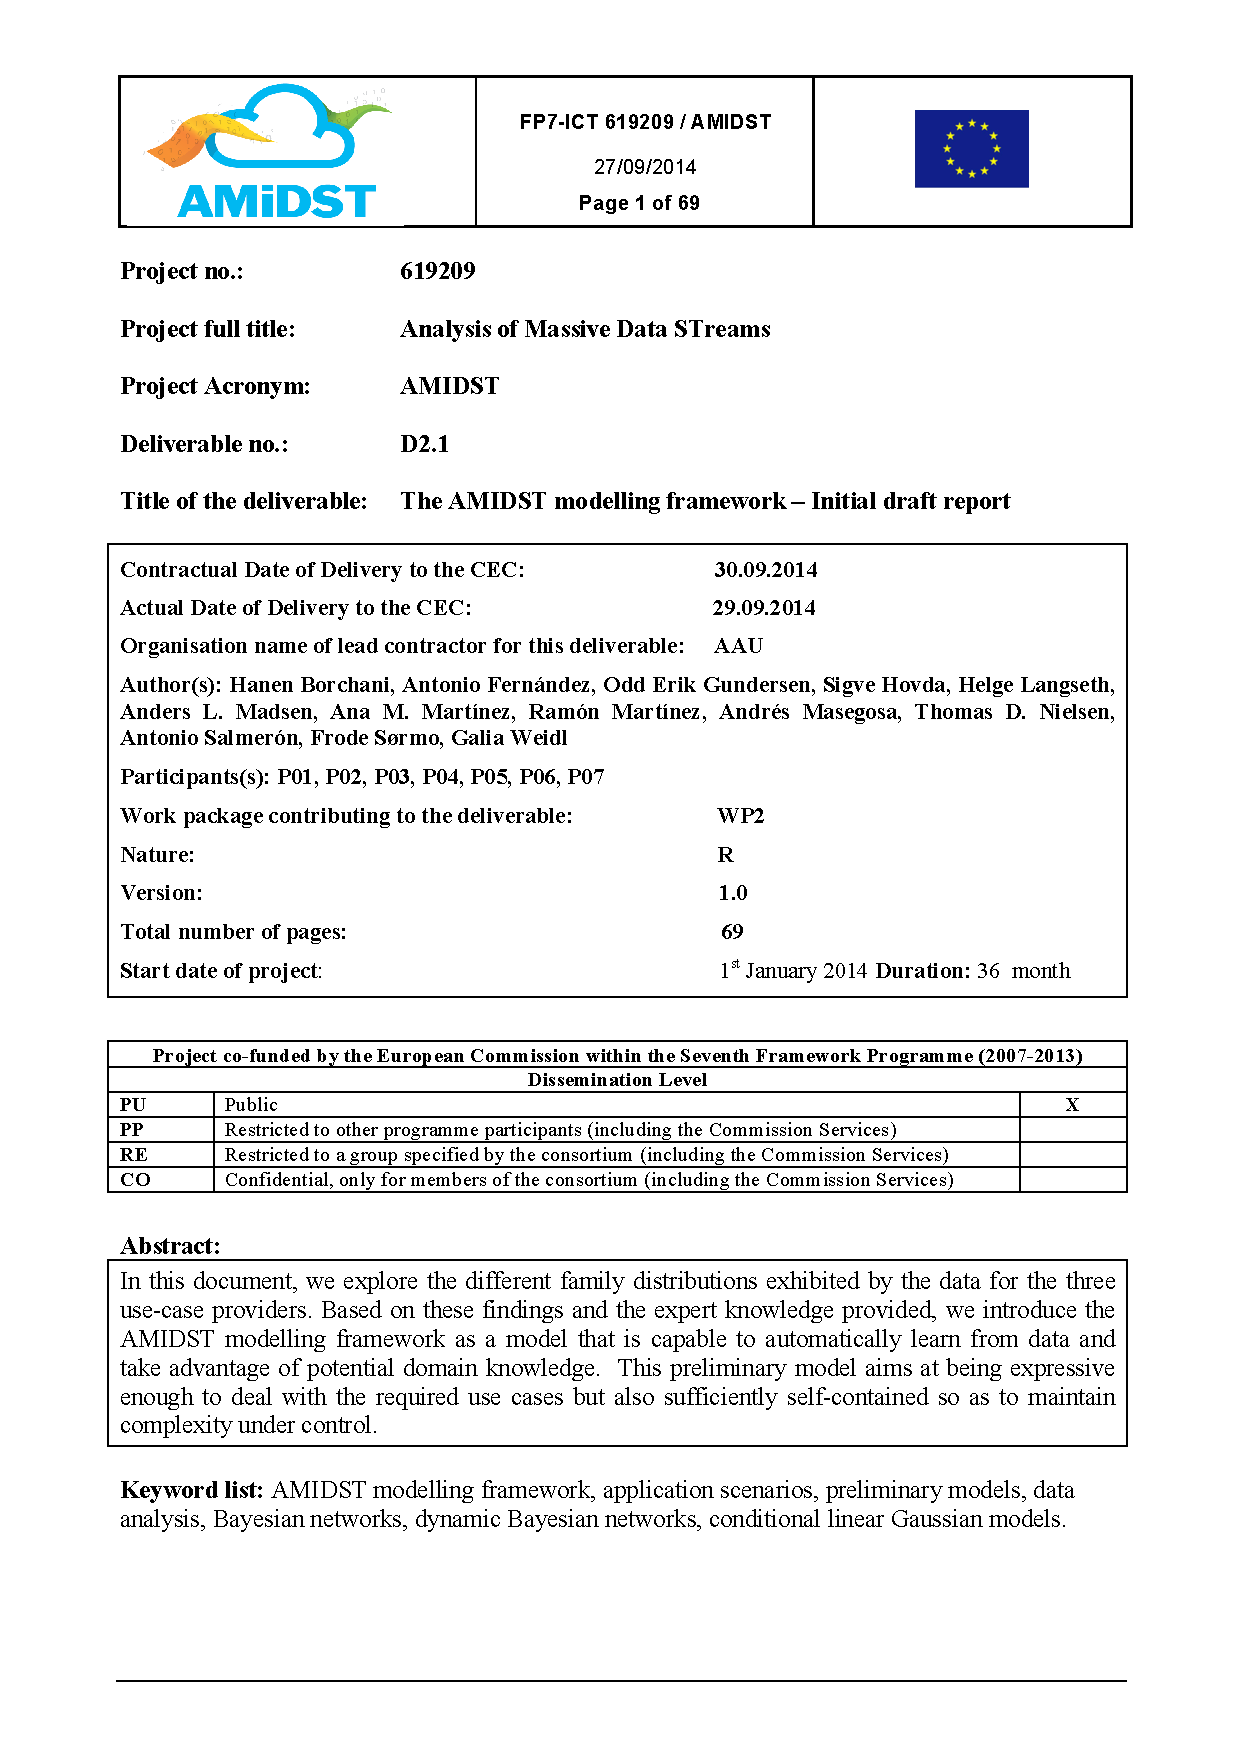
\includepdf[pages={1}]{figures/FrontPage.pdf}
%\newpage\null\thispagestyle{empty}\newpage

% Table of contents
\tableofcontents

\newpage

% Document History

\section*{Document history}

\begin{table}[htbp]
  \centering
  \begin{tabularx}{\linewidth}{|p{13mm}| p{18mm}| X | X |} \hline
    {\bf Version} & {\bf Date} & {\bf Author (Unit)} & {\bf Description} \\ \hline
    v0.3 &  &  & The test and evaluation framework discussed and established \\ \hline
    v0.6 &  &  & Initial draft finished and reviewed by the PSRG  \\ \hline
    v1.0 &  & & Final version of document  \\ \hline
  \end{tabularx}
\end{table}

\newpage

\section{Executive summary}

This document is by no means ready, so I haven't written anything here. 

\newpage

% Introduction
\section{Introduction}

Even though the number of algorithms designed for learning on streaming data is increasing, there is still not a unified and well accepted way for evaluating them.  This is because testing and evaluating algorithms that are designed to work on streaming data are more difficult those designed to work on static data.  There are both statistical and computational reasons for this.  

Static data is data, where each instance can be assumed to be identically and independently distributed i.i.d.  On streaming data, one can often not assume that data instances are i.i.d.  Moreover, the algorithms are often designed to weight measurements that are close to the actual time step higher than measurements that are further back.  On streaming data, we must therefore assume that data are generated from underlying distributions that are time dependent and also that the algorithms themselves are time dependent.  

Computational challenges are related to the fact that the data come from an open-ended data stream, conceptually infinitely long, which imposes practical challenges related to restrictions on cpu-time and memory allocation.  

Various error measures related to stream data has been proposed in the papers of Gama et. al. \cite{Gam09}, \cite{Gam09_2}, \cite{Gam12}.  A loss function is typically related to the penalty of misclassifications on classification problems or residuals in regression models.  The holdout error is basically the average loss on a holdout dataset of fixed size.  The predictive sequential, or \emph{prequential} error is defined as the average loss function up to time step $i$, where $i$ is the current time step.  Moreover, it was also suggested to use a prequental error measure, which involved a forgetting factor such as using a time window or fading factors.  In paper \cite{Gam12}, convergence towards the Bayes error was shown for all these performance measures provided that the learners are consistent and data are i.i.d.  Moreover, it was shown that if data was allowed to drift over time, meaning that samples are only locally i.i.d, then the prequental error measures with forgetting mechanisms were favourable.

\todo{Relate to other work on streaming data as well.}

The applications that are covered in this report have different characteristics than the applications discussed in \cite{Gam12}.  Some problem will be evaluated on a holdout dataset assuming i.i.d and a stationary algorithm.  Other problems can not assume i.i.d on a local scale, but stationarity can be assumed on a larger time scale.  

In this paper we will establish formal procedures for testing and evaluating the developed models and algorithms. This includes specification what metrics are relevant to use to quantify the ability of the AMIDST system, such as relevant formalization of loss functions, maximum response-times, memory limits and output format.  The paper will also include 
considerations about what quantitative improvements AMIDST should obtain over state of the art.

In section \ref{sec:methodology}, AMIDST relevant methodologies for evaluation of both batch and streaming algorithms are identified and discussed.  This section forms the foundation of the subsequent sections, where the exact evaluation routines for each use case provider is given. These sections contains a description of the requirements related to evaluation as described in Delivery 1.2, a short description of the algorithms and the data and finally methods for evaluating predictive and runtime performances.  Section \ref{sec:conclusion} concludes the report.


%\quote{\emph{Task description: In this task we will establish formal procedures for testing and evaluating the
%    developed models and algorithms. This includes specification of maximum response-times, output format,
%    relevant formalization of loss functions, investigations into what metrics are relevant to use to quantify
%    the ability of the AMIDST system, and considerations about what quantitative improvements AMIDST should
%    obtain over state of the art.}}
%
%
%From Helge's slides at the WP 3 kickoff meeting:
%\begin{itemize}
%\item Massive datasets: find relevant techniques, ensure scalability, etc.
%\item Online evaluation of streams: find relevant techniques, ensure scalability, define behavior in changing environment, etc.
%\item Significance of results, e.g., considering changing environment vs. ``reproducability'', distribution for test-statistic, significance levels/sizes of test-sets, etc.
%\end{itemize}


% Test and evaluation methodology
% !TEX root = deliverable1.3.tex
\section{Test and evaluation methodology}
\label{sec:methodology}

As discussed in the introduction, finding appropriate performance measures on streaming data is more difficult than finding performance measures on non streaming data.  We will therefore start by discussing some relevant performance measures for classification of i.i.d. non streaming data. 

\subsection{Performance measures for classification on i.i.d. data}
\label{sec:static}

Consider a dataset of fixed size $n$, where each instance is independently drawn from a joint probability distribution $P(\bmX,Y)$,. Here  $\bmX$ and $Y$ are random variables; $\bmX$ is known as the explanatory variable and $Y$ is the class label.  These two variables have output spaces $\Omega_X$ and $\Omega_Y$, respectively.
In classification, we typically consider a hypothesis function $h: \, \Omega_X \rightarrow \Omega_Y$, where $\Omega_Y$ is a finite set of class labels; note that $\Omega_Y=\{0,1\}$  for a binary classification problem.
 $\Omega_X$ is a space of all possible explanatory vectors.  
In terms of evaluating the performance of $h$, we use a dataset of input-output pairs $(\bmx_i, y_i)$ that are independently drawn from $\Omega_X  \times \Omega_Y$. 
The result of such an experiment can be shown in a confusion matrix.  An example of a confusion matrix is shown \tabref{catdograbbit}, where the classifier is attempting to distinguish cats, dogs and rabbits. 

\vspace{1ex}
\begin{table}[ht]
\centering
\begin{tabular}{ll|r|r|r|}
\cline{3-5}
&&  \multicolumn{3}{c|}{Predicted class}\\
\cline{3-5}
&& Cat & Dog & Rabbit\\ 
\cline{1-5}
\multicolumn{1}{ |c| }{\multirow{3}{*}{Actual class} }
 & Cat & 5 & 3& 0\\
\cline{2-5}
\multicolumn{1}{ |c| }{} & Dog & 2 & 3 & 1\\
\cline{2-5}
\multicolumn{1}{ |c| }{} & Rabbit & 0 & 2 & 11\\
\cline{1-5}
\end{tabular}
\caption{Example of a confusion matrix.  A classifier is labelling instances as either cats, dogs or rabbits.  The accuracy is the sum of the diagonal elements divided by the total number (in this case 19/27).}
\label{tab:catdograbbit}
\end{table}
\vspace{1ex}

A global measure of the classification algorithm is the classification accuracy which is calculated as the sum of the diagonal elements divided by the sum of all numbers in the table (in this case 19/27).  
It is important to note that the accuracy is not telling the whole story of the classification rule.  
For instance, by looking at the table it is seen that the algorithm distinguishes cats from rabbits quite easily, but it is much harder to distinguish cats from dogs.  This property cannot be realized by looking at the accuracy alone.  

Moreover, accuracy is also very dependent on how evenly the classes are distributed.   For instance, when there are a lot more instances of one class compared to the others, a naive classification rule that always predict the majority class will get a high accuracy, even though the method is not using any of the information that is contained in the explanatory variables.  
These are reasons for inspecting the full confusion matrix for interpreting the classification rule.  

In order to inspect various properties of a classification rule, various performance measures can be calculated from the confusion matrix.  We have decided to limit this exposition to binary classification, while being aware that most of the performance measures can be expanded to discuss multi class classifiers.

For a binary classifier, such as classifying cats and non-cats, the confusion matrix is of size two - by - two; an example is shown in \tabref{binary}.  
It is common to introduce positives and negatives  instead of the class labels.  
A true positive is therefore an actual cat that has been predicted to be a cat, while false positives, true negative and false negatives are defined in an equivalent manner.  


\vspace{1ex}
\begin{table}[ht]
\centering
\begin{tabular}{ll|r|r|}
\cline{3-4}
&&  \multicolumn{2}{c|}{Predicted class}\\
\cline{3-4}
&& Cat & Not cat\\ 
\cline{1-4}
\multicolumn{1}{ |c| }{\multirow{3}{*}{Actual class} }
& Cat & 5 & 3\\
\cline{2-4}
\multicolumn{1}{ |c| }{} & Not cat & 2 & 17 \\
\cline{1-4}
\end{tabular}
\caption{Example of a confusion matrix for a classifier of cats and not cats. The accuracy is 22/27.}
\label{tab:binary}
\end{table}
\vspace{1ex}

\vspace{1ex}
\begin{table}[ht]
\centering
\begin{tabular}{ll|r|r|}
\cline{3-4}
&&  \multicolumn{2}{c|}{Actual Condition}\\
\cline{3-4}
&& Positive & Negative\\ 
\cline{1-4}
\multicolumn{1}{ |c| }{\multirow{3}{*}{Test outcome} }
& Positive & 5 & 2\\
\cline{2-4}
\multicolumn{1}{ |c| }{} & Negative & 3 & 17 \\
\cline{1-4}
\end{tabular}
\caption{Example of a confusion table for a classifier of cats and not cats. The true positives and true negatives are on the diagonal, while the two other numbers are the false positives and the false negatives.}
\label{tab:confusionTable}
\end{table}
\vspace{1ex}

The results are commonly shown in a confusion table (see \tabref{confusionTable}), which is not the same as a confusion matrix.  From a confusion table it is easy to calculate numerous numbers that describes the classification rule.  Specifically, we mention the true positive and false positive rates.  True positive rates, also known as recall, is the number of true positives divided by the total number actual positives.  The false positive rates, also known as fall-out, is the number of false positives divided by the total number actual positives. 
By investigating various numbers that can be deduced from the confusion table, it is possible to discuss classification rules, even when the datasets are unevenly distributed.  That is, when some class label have more instances than others.

However, these numbers do not take into account that some misclassifications might be more costly than others.  For instance, a false positive might be more costly than a false negative.  For instance in the case of diagnosing cancer, it might be more costly to not treat a person that is sick, compared to treating a healthy person.  Moreover, the cost of each false positive (or false negative) may not be constant either.  For instance, if the classifier is predicting whether a client in a bank will default a loan or not, the cost is clearly related to the size of the loan in question.  The next subsection includes a procedure to include such costs in a performance measure.

\subsubsection{Empirical risk}
\label{sec:empRisk}

In mathematical optimization, statistics, decision theory and machine learning, a loss function or a cost function is a function that maps an event or values of one or more variables onto a real number that is intuitively representing some \emph{cost} associated with the event. Loss functions can be used on optimization problems, when an algorithm or a method is optimized by minimizing the loss function.  Moreover, loss functions are frequently used to diagnose and compare various algorithms or methods.  
We define the \emph{loss function} as a real and lower-bounded function $L$ on $\Omega_X \times \Omega_Y \times \Omega_Y$.  In the case of classification, the value of the loss function at an arbitrary point $(x, h(\bmx), y)$ is interpreted as the loss, or cost, of taking the decision $h(\bmx)$ at $\bmx$, when the right decision is $y$.  Notice that the loss function is defined to also depend on $\bmx$.  This is of high practical use, because a certain misclassification might be more expensive than another. 

In the frequentist perspective, the expected loss is often referred to as the risk function \cite{Vap00}.  It is obtained by taking the expected value over the loss function with respect to the probability distribution $P(\bmX,Y): \Omega_X\times \Omega_Y \rightarrow \mathbb{R}^+$.  The \emph{risk function} is given by

\begin{equation}
\label{def:risk}
R(h) = \int_{\Omega_X,\Omega_Y} L(x,h(\bmx),y) dP(\bmx,y).
\end{equation}

In the case when the costs are independent of $x$ and also that there is no cost related to correct classification, the risk function reduces to the well known expected cost of misclassification (ECM)

\begin{equation}
\label{eq:ecm}
ECM =  c(1|0)p(1|0)p_0  + c(0|1)p(0|1)p_1.
\end{equation}
Here, $c(1|0)$ is the cost for misclassifying an item of class zero as class one and $p(1|0)$ is the misclassification probability given class zero.  The quantities $c(0|1)$ and $p(0|1)$ are defined equivalently, while $p_0$ and $p_1$ are the priors.  

In general, the risk $R(h)$ cannot be computed because the distribution $P(\bmX,Y)$ is unknown.  However, we can compute an approximation, called empirical risk, by averaging the loss function on the data set $\calD$ of size $N$, where each element in $\calD$ is $(\bmx_i, y_i)$.  The empirical risk is given by 

\begin{equation}
\label{def:empRisk}
R_{emp}(h, \calD) = N^{-1} \sum_{i=1}^N L(x_i, h(\bmx_i), y_i).
\end{equation}

Many supervised learning algorithms are optimized by finding the $h$ in a hypothesis space $\mathcal{H}$ that minimizes the empirical risk on a data set that is used only for training the classification rule.  In this case, a separate data set is needed for testing the classifier.  In this document, we focus only on testing classifiers.  We only use empirical risk to quantitatively describe the methods.

\subsubsection{Evaluation of families of classification rules}
\label{sec:hypothesisSpace}

So far we have discussed how to evaluate a single classification rule.  
However, probabilistic classifiers operate by calculating the probability distribution $P(Y\given\bmx)$, and then comparing this probability to a certain threshold.  
We will call this estimated probability the output function $q: \Omega_X \rightarrow \mathbb{R}^+$.  In the probabilistic framework the range of $q$ is $[0, 1]$, but this restriction is not necessary for this theory to be well-defined.  
The potential classification rules are the family of hypothesis functions $\mathcal{H}$, where each element $h_T:\Omega_X \rightarrow \Omega_Y$ has the form 

\begin{equation}
\label{eq:ht}
h_T(\bmx) = 
\begin{cases}
0 \quad \mbox{if} \quad q(\bmx) \leq T\\
1 \quad \mbox{otherwise.}
\end{cases}
\end{equation}

It is of interest to evaluate all these classification rules.  The receiver operating characteristic (ROC) is a plot of the true positive rate as a function of the false positive rate, as the threshold $T$ varies over all relevant values.  An example is seen in figure \ref{fig:ROC}.

\begin{figure}[ht!]
\centering
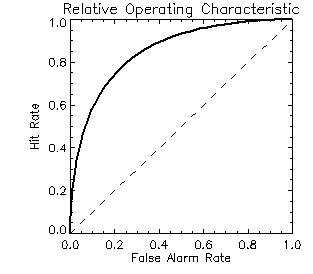
\includegraphics[scale=0.70]{figures/ROC.png}
\caption{\label{fig:ROC} Receiver operating characteristics curve.  True positive or hit rate is shown as a function of false positive or false alarms rate.  The dashed line shows the ROC curve of the random guess.}
\end{figure}


The ROC curve allows a visual exposition of the family of classifiers $\mathcal{H}$, in the sense of true positive rates and false positive rates.  In particular, it is easy to see which threshold is needed for a certain hit rate or true positive rate.  This plot is clearly independent on class distributions and the whole cost content.

Moreover, it is also of interest to reduce all this information into a single number.  The area under the ROC curve, also known as AUC, is such a number.  
AUC is independent of $T$. The AUC is a popular method for evaluating classification problems where class imbalance is vital, because it is invariant to the class distribution. 
AUC has the statistical interpretation that it is the probability that a random member of the ``positive'' class is scored higher than a random member of the ``negative'' class.  
AUC is therefore a measure of the \emph{ranking ability} of the output function.  
This is particularly relevant if one wants to change the classification threshold as a consequence of changing class distributions or  changing misclassification costs \cite{Wu07}.  
Moreover, it has also been pointed out that AUC is more preferable than accuracy for model evaluation \cite{Gam10}.  



%It may be difficult to comprehend what AUC is at this point, but we will return to it afterward.

We will now discuss the underlying statistical properties of AUC. First, let $\bmX_0$ and $\bmX_1$ be random variables with probability distributions $P(\bmX | Y = 0)$ and $P(\bmX | Y = 1)$, respectively.  We define the random variables $Q_0 = q(\bmX_0)$ and $Q_1 = q(\bmX_1)$.  To summarize, $Q_0$ is basically the output value you get when you pick a random sample of class zero and calculate the probability for it to be a member of class one; similarly for $Q_1$.  

The probability $P(Q_1 > Q_0)$ is of interest, because this says what is the probability that if you take one sample by random from each of the populations, what is the chance that the output value from sample one is higher than the output value of sample zero.  This question is independent of $T$, meaning that the discussion about priors and costs are not needed. This probability is called the concordance probability.

Without exposing the details, it is possible to show that
\begin{equation}
\label{eq:concurrent}
\mbox{AUC} = P(Q_1 > Q_0).
\end{equation}
It is important to note that nothing need to be assumed about the probability distributions of $Q_0$ and $Q_1$.  Furthermore, it is worth noting that the concordance probability is exactly equal the common language effect size of the Mann-Whitney $U$ test.  We discuss the Mann-Whitney $U$ test next.

\subsubsection{Mann-Whitney $U$ test}
\label{sec:U}

The Mann-Whitney $U$ test  \cite{Man47} is a nonparametric test of the null hypothesis that two populations are the same against an alternative hypothesis where one population tends to have larger values than the other.  It is the nonparametric version of common $t$-test, where both populations are assumed to be of normal distributions.  It is nearly as efficient as the $t$-test on normal data and far more efficient on non normal data.  In our context, we can use the Mann-Whitney $U$ test to discuss whether values of $Q_1$ are consistently larger than values of $Q_0$.  

A relevant assumption for our problem is that all samples of $Q_0$ and $Q_1$ are assumed to be independent of each other.  On stationary streams, we know this is not true as two consecutive measurements are clearly dependent.  However, in the context of interpretation, we can imagine that the samples of randomized.  

A more important assumption is that under the null hypothesis, the probability distributions of $Q_0$ and $Q_1$ are exactly equal, while the alternative hypothesis is that the distributions have different means, but similar shapes.  It is clearly a problem if for instance $Q_0$ is one sided exponentially distributed, while $Q_1$ is normally distributed with a larger mean.   
Other assumptions can be stated for this test as well.  A more thorough discussion can be found in \cite{Fay10}.

We define a data set $\calD$ with $n$ input-output pairs $(x_i, y_i)$, independently drawn from $P(\bmX,Y)$.  From the data set we have two populations $\bmq_0 = \{q(\bmx_i) , | \, y_i = 0 \}$ and $\bmq_1 = \{q(\bmx_i) , | \, y_i = 1 \}$.  Their sizes are $n_0$ and $n_1$ so that $n_0 + n_1 = n$.  Calculating the $U$ statistics is straightforward, where these two values are obtained 

\begin{equation}
\label{eq:U}
U_0 = \sum_{i=1}^{n_0}\sum_{j=1}^{n_1} H(\,q_{1,j} - q_{0,i}    \,) \quad \mbox{and} \quad 
U_1 = \sum_{i=1}^{n_0}\sum_{j=1}^{n_1} H( \,q_{0,i} - q_{1,j}    \,).
\end{equation}
Here, $H(\cdot)$ is the heaviside step function and notice that $U_0 + U_1 = n_0n_1$.  For large samples, each $U$ ($U_0$ or $U_1$) is approximately normally distributed. In that case, the standardized value

\begin{equation}
\label{eq:z}
z = \frac{U_0 - m_{U}}{\sigma_{U}},
\end{equation}
where $m_U$ and $\sigma_U$ are the mean and standard deviation of $U$ given by

\begin{equation}
\label{eq:z}
m_U = \frac{n_0n_1}{2} \quad \mbox{and} \quad 
\sigma_U = \sqrt{\frac{n_0n_1(n_0 + n_1 + 1)}{12} }.
\end{equation}

Significance of test can be checked in tables of the normal distribution.  Although, such an hypothesis test is interesting by itself, we are more interested in the concordance probability $P(Q_1 > Q_0)$ which is defined by

\begin{equation} 
\label{eq:concordance}
P(Q_1 > Q_0) = \frac{U_1}{n_0n_1}.
\end{equation}

It is important to note that even though the Mann-Whitney $U$ test is dependent on whether the shapes of the probability distributions of $Q_0$ and $Q_1$ are similar, this requirement is not necessary for the concordance probability.  To be more explicit, the problem when $Q_0$ is for instance one sided exponentially distributed and $Q_1$ is normally distributed, is not a violation of preliminary assumptions.  

The concordance probability or AUC are therefore a measure of the ranking ability of the output function.  The Mann Whitney $U$-test allows one to test whether the result that is obtained is not just be chance in the way the data set is drawn.  It can also be used for designing experiments in terms of reasoning about how large data sets are needed for making an effective test.

Moreover, equation \eqref{eq:concordance} shows a simple way of calculating $P(Q_1 > Q_0)$ and AUC.

\subsubsection{Multi class classification}

In the case of estimating the empirical risk equation \eqref{def:empRisk} is valid for multi class classification as well.  The AUC measure is generally defined for binary classification.  However, an extension of AUC to multi class problems is fo4iund in \cite{Han01}.  If we let AUC($i,j$) be the AUC between class $i$ and $j$, where samples that do not belong to either $i$ or $j$ are ignored, then the multi class AUC is defined as 


\begin{equation} 
\label{eq:multiAUC}
\mbox{AUC}_m = \frac{1}{m(m-1)}\sum_{i,j} AUC(i,j),
\end{equation}
where $m$ is the number of classes.  It is worth noting that all AUC($i,i$) are equal to zero. This is basically the same as averaging all possible binary AUC.  This extension to multi class classification on streaming data is straightforward and will not be repeated each time in the next section.

\subsection{Performance measures for classification on streaming data}
\label{sec:stream}

This section includes various evaluation methods for classification on data streams.  Central to choices of evaluation methods are stationarity versus concept-drift, class imbalance, whether a scoring function exists, computational constraints and also the importance of early detection when a data stream changes behaviour.

\subsubsection{Stationary data streams}
\label{sec:stationary}

Let $\{X_{t}\}$ be a stochastic process, where $p_X(\bmx_{t_1 + \tau},...,\bmx_{t_k + \tau} )$ is the probability distribution function of the joint distribution at $t_1 + \tau,...,t_k + \tau$.  Then $\{X_t\}$ is a stationary process, or a stationary stream, if, for all $k$, for all $\tau$ and for all $t_1 + \tau,...,t_k + \tau$, 

\begin{equation}
\label{eq:stationarity}
p_X(\bmx_{t_1 + \tau},...,\bmx_{t_k + \tau} ) = p_X(\bmx_{t_1},...,\bmx_{t_k} ),
\end{equation}
where the $\bm{x_t}$s are vectors of fixed size.  Clearly, $p_X(\cdot)$ is not a function of time.  

In stationary streams, the mean and the variance, if they exist, do not vary.  The covariance structures to neighboring instances are also preserved.  To summarize, stationary streams are more general than i.i.d. streams, where the covariance to all other instances are zero.  

In \cite{Gam13}, the prequential empirical risk is defined as 

\begin{equation}
\label{eq:prequentialRisk}
R_{emp}(h, \{X_{t_k}\}) = k^{-1} \sum_{i=1}^k L(\bmx_{t_i} , h(\bmx_{t_i} ), y_{t_i}),
\end{equation}
where $y_{t_i}$ is the class label at time $t_i$ and $n$ is the number of samples up to $t_k$.  In the original paper, the notation is different and the measure is called the prequental error  Adaptations are made to comply with notation and definitions in section \ref{sec:static}.  Notice, that the loss function in the prequential empirical risk, is generalized compared to \cite{Gam13}, to also include dependency of $\bm{x_{t_i}}$, which may in fact be just $t_i$.  This generalization means that it is possible to model evolving loss as well.

\drop{\todo{Sigve says: Include a discussion of statistical interpretation of loss functions on stationary data.  Dependence between timesteps is essential. Is this a problem? What opportunities do we have with evolving loss? Maybe nothing, but worth reflecting on.}}

AUC is also popular in a streaming context, in the case when the classification is based on a scoring function, which is common for Bayesian networks. 
Specialized learning algorithms for imbalanced streams are proposed in \cite{Dit13, Hoe12, Lic10}, where it is also pointed out that this problem is particularly difficult and effective algorithms for evaluation is vital.  
AUC is calculated on limited holdout sets are used in  \cite{Dit13, Lic10}, while AUC is calculated on the entire stream in  \cite{Hoe12}. If the whole stream is used, it may have computational problems related to memory and cpu time.  

The prequential AUC at time step $t_k$ can be calculated by
\begin{equation}
\label{eq:prequentialAUC}
\mbox{AUC}_{t_k}= \frac{U_{1,k}}{n_{0,k}n_{1,k}},
\end{equation}
where $n_{0,k}$ and $n_{1,k}$ are the number of negatives and positives up to $t_k$.  To be precise, $n_{0,k} + n_{1,k} = k$.  The quantity $U_{1,k}$ is calculated by the second $U$-statistic as of equation \eqref{eq:U} (using $n_{0,k}$ and $n_{1,k}$).

On a data stream there is an opportunity of calculating AUC recursively with the following algorithm.

\begin{equation}
\label{eq:prequentialAUC2}
U_{1,k}= 
\begin{cases}
U_{1,k-1} + \sum_{j=1}^{n_{1,k}} H( \,q_{0,n_{0,k}} - q_{1,j}    \,)
 \quad &\mbox{for} \quad y_{t_k} = 0\\
U_{1,k-1} + \sum_{i=1}^{n_{0,k}} H( \,q_{0,i} - q_{1,n_{1,k}}    \,)
\quad &\mbox{for} \quad y_{t_k} = 1.\\
\end{cases}
\end{equation}
Clearly AUC calculation is $O(k)$, which might be a problem for very long streams.  

Another method for calculating AUC  involves sorting the scores of all instances and iteration over this list. It is essential that the sorted list always keeps the mapping from each score to either a positive or a negative.  At each time step, the list of scores, the number of positives and the number of negatives are updated.  The AUC is calculated by algorithm \ref{AUCalg}.  This method is also $O(k)$.

\begin{algorithm}[H]
 \KwData{$s$: Current score, $sortedList$: sorted list of all scores in a stream, $p$: number of positives in sorted list, $n$: number of negatives in sorted list}
 \KwResult{Prequential $AUC$ at the current time step}
$sortedList.update(s)$;\\
$p.update(s)$;\\
$n.update(s)$;\\
$c \leftarrow 0, AUC \leftarrow 0$;\\
\ForAll{scores $t \in$ sortedList}{
\If{isPositive($t$)}{
$c \leftarrow c + 1$
}\Else{
$AUC = AUC + c$;
}
}
$ AUC = AUC/(p \cdot n)$;
\label{AUCalg}
 \caption{Calculation of prequential AUC at each time step in a stream.  Here, $sortedList.update(s)$ takes in the current score $s$ and places it correctly in the sorted list. The method $isPositive(s)$ computes whether the score $s$ is positive or not, while $p.update(s)$ and $n.update(s)$ updates the number of positives $p$ and negatives $n$.}
\end{algorithm}

It is worth noting a few points about the statistical interpretability of AUC on stationary streams.  Unless the stream is also i.i.d. the $q_{0,i}$s and the $q_{1,i}$s are generally dependent on neighboring points.  This fact is however not contradicting the fact that AUC is equal to the concordance probability $ P(Q_1 > Q_0)$.  This is because the definitions of $Q_0$ and $Q_1$ are $Q_0 = q(X_0)$ and $Q_1 = q(X_1)$ and 
that $X_0$ and $X_1$ are random variables with probability distributions $P(X | Y = 0)$ and $P(X | Y = 1)$.  The key point is that $P(X | Y = 0)$ and $P(X | Y = 1)$ are not dependent on time in stationary streams.  This is not true on non stationary streams.  

\drop{In practice, samples of $Q_0$ and $Q_1$ can be though of as picking samples from $\bv{q_0}$ and $\bv{q_1}$, respectively.}

\subsubsection{Data streams that involve concept-drift}

Concept drift is generally understood as unforeseen changes in statistical properties of the target variable.  In the case of regression this can basically be understood as non stationary of the dependent variable.  In the case of classification, it is understood as the class distribution is \emph{not} constant in time.  

However, this definition is not always clear cut in the literature.  For instance in \cite{Brz14}, concept drift is understood broader, where non stationarity of explanatory variables are present in addition to time dependent class distributions.   For clarity, in this paper we refer to concept drift in the sense of \cite{Brz14}.

In \cite{Gam13}, two estimators are suggested for dealing with concept drift and/or non stationary explanatory variables.  The first estimator involves calculating the prequential empirical risk over a sliding window of $w$ samples. 

\begin{equation}
\label{eq:prequentialRisk2}
R_{emp}(t_k, \{h_{t_k}\}, \{X_{t_k}\}, w) = w^{-1} \sum_{i=k - w +1}^k L(\bmx_{t_i} , h_{t_i}(\bmx_{t_i} ), y_{t_i}).
\end{equation}
Notice that $R_{emp}(t_k, \{h_{t_k}\}, \{X_{t_k}\}, w)$ is a function of time and not just a single number.  Hence, the measure reflects the expected loss at $t_{k-\mbox{floor}(w/2)}$.  Notice also that the classification rule itself $h_{t_i}$ is allowed to be a function of time.

The second estimator involves fading factors and is defined as follows

\begin{equation}
\label{eq:prequentialRisk3}
R_{emp}(t_k, \{h_{t_k}\}, \{X_{t_k}\}, \alpha) =\frac{\sum_{i=1}^k \alpha^{i-k}L(\bm{x_{t_i}} , h_{t_i}(\bm{x_{t_i}} ), y_{t_i})}{\sum_{i=1}^k \alpha^{i-k}} \quad \mbox{where} \quad 0 \leq \alpha \leq 1.
\end{equation}
When $\alpha$ is equal to one, this reduces to the prequental empirical risk with no forgetting factor, while in the case when $\alpha$ is equal to zero, the estimator forgets all effects before $t_k$.

In the special case when the loss function is zero-one and $h$, or $h_k$, is consistent, then it is shown in \cite{Gam13} that 
$R_{emp}(t_k, \{h_{t_k}\}, \{X_{t_k}\}, \alpha)$, $R_{emp}(t_k, \{h_{t_k}\}, \{X_{t_k}\}, w) $ and $R_{emp}(h, \{X_{t_k}\})$ approximates the Bayes error in the limiting cases.

As said in \ref{sec:stationary}, $P(X | Y = 0)$ and $P(X | Y = 1)$ are not dependent on time in stationary streams. However, in our definition of concept-drift, which includes non stationary explanatory variables, $P(X | Y = 0)$ and $P(X | Y = 1)$ are generally dependent on time.  This means that an AUC that is calculated by either equation \eqref{eq:prequentialAUC2} or algorithm \ref{AUCalg} at the current time step, may be severely biased by very old measurements.

To overcome this problem, it is suggested in \cite{Brz14}, a prequantial AUC with a forgetting factor.  The method involves calculating AUC on a sliding window of fixed size in a similar manner as algorithm \ref{AUCalg}.  This algorithm is explained in algorithm \ref{AUCalg2}.

\begin{algorithm}[H]
 \KwData{$s$: Current score, $sortedList$: sorted list of scores in the sliding window, $p$: number of positives in sorted list, $n$: number of negatives in sorted list}
 \KwResult{Prequential $AUC$ at the current time step}
$sortedList.update(s)$;\\
$p.update(s)$;\\
$n.update(s)$;\\
$c \leftarrow 0, AUC \leftarrow 0$;\\
\ForAll{scores $t \in$ sortedList}{
\If{isPositive($t$)}{
$c \leftarrow c + 1$
}\Else{
$AUC = AUC + c$;
}
}
$ AUC = AUC/(p \cdot n)$;
\label{AUCalg2}
 \caption{Calculation of prequential AUC at each time step in a stream.  Here, $sortedList.update(s)$ takes in the current score $s$ and throws out the oldest score before resorting the list. The method $isPositive(s)$ computes whether the score $s$ is positive or not, while $p.update(s)$ and $n.update(s)$ updates the number of positives $p$ and negatives $n$.}
\end{algorithm}

\drop{\todo{Sigve says: Maybe discuss stationary explanatory variables with consept drift versus non stationary explanatory variables with concept drift.}}

\subsubsection{Risk related to early and late warnings}

When working on data streams it may sometimes be of interest to give as early warnings as possible.  Another way of saying this is to penalize late warnings more and more.  We therefore suggest this measure, where the notation is the same as in equation \eqref{eq:prequentialRisk2}

\begin{equation}
\label{eq:prequentialRisk3}
R_{emp}(t_k, \{h_{t_{k+m}}\}, \{X_{t_k}\}, w) = w^{-1} \sum_{i=k - w +1}^k L(\bmx_{t_i} , h_{t_{i+m}}(\bmx_{t_i} ), y_{t_{i+m}}).
\end{equation}
Here, $m$ denotes some time steps into the future and $h_{t_{k+m}}$ denotes prediction at $t_{k+m}$.
\todo{Sigve says: Reflect more and relate to Cajamar. Helge has promised to help out.}


%
%In the use case scenarios in the AMIDST software, all problems are binary classifiers, which involve dividing the streams into sub streams that are labeled as either positives or negatives.  There are two important approaches here.
%
%The first approach deals with multiple streams and the global time dependence is removed by sampling all these streams into multiple sub streams, which are starting and ending at the same time steps.  Each sub stream is labeled as either a positive or negative based on the data at the end time.  An evaluation time step that is a fixed between the start and the end is also defined.  The explanatory variables are derived from the data between the start and the evaluation time step.  In this sense, the data is basically i.i.d.
%
%The second approach is when there is basically one stream where one can assume stationarity on a global scale.  Sub streams with large enough distance to other sub streams are taken out of the stream.  These sub streams are labeled as either a positive or a negative.  For instance, a positive is when something is happening towards the end of the sub stream, while a negative is a sub stream where nothing happens.  When the AMIDST software run, the output function is evaluated at each time step.  Depending of the problem, a heuristic algorithm is chosen to output a single number for each sub stream based on the output values.  This can for instance be the maximum value of the output function on an interval that is prior to an event.  
%





 

%\emph{Here we should cover general methods for doing test and evaluation of models in a streaming
%  context. These methods will subsequently be instantiated in relation to the three use case providers so I
%  guess that we should primarily consider the methods that are directly related to the needs of the use case
%  providers, but (taking the back ground of one of the reviewers into account) we might probably benefit from
%  going a bit beyond the immediate needs and put all this stuff into a broader context ...}
%
%\cite{Kap14}, \cite{Gam09}, \cite{Gam09_2}, \cite{Gam13}, 


% Use cases: test and evaluation
%\section{Use case specific test and evaluation}

% !TEX TS-program = pdflatex
\documentclass{article}

\usepackage{hl_short}
\usepackage{times}
\usepackage{graphicx}
\usepackage{latexsym}

\usepackage{bm}
\usepackage{amsbsy}
\usepackage{amsmath}
\usepackage{amsfonts}
\usepackage{amssymb}

\usepackage{subfigure}
\usepackage{color}

\usepackage{theorem}

\theoremstyle{theorem}
\newtheorem{theorem}{Theorem}

\usepackage{array}

\theoremstyle{definition}
\newtheorem{definition}{Definition}
\newtheorem{remark}{Remark}

\newcommand{\bu}[1]{\mathbf{#1}}
\newcommand{\bv}[1]{\bm{#1}}


\newcommand{\W}{\mathbf{W}}
\newcommand{\X}{\mathbf{X}}
\newcommand{\Y}{\mathbf{Y}}
\newcommand{\Z}{\mathbf{Z}}
\newcommand{\w}{\mathbf{w}}
\newcommand{\x}{\mathbf{x}}
\newcommand{\y}{\mathbf{y}}
\newcommand{\z}{\mathbf{z}}
\newcommand{\argmax}[1]{\underset{#1}{\operatorname{arg}\,\operatorname{max}}\;}

\newcommand{\comment}[1]{ \begin{center}{\bf [[ #1 ]]}\end{center}}

\title{Practical Considerations for Testing the Cajamar Use Case}
\author{Sigve, Helge, Thomas}
\date{\today}


\begin{document}
\maketitle


\section{Cajamar: Test and evaluation}

This section introduces the testing procedures for the Cajamar use cases. Bla bla. Bla bla. 

\subsection{Use-case requirements}

The test and evaluation procedures for Cajamar will be developed along the lines introduced in Deliverable 2.1: Instead of testing use cases separately, we utilize the notion of {\em application scenarios}. 
An application scenario is a defined by a sequence of use cases that combined constitutes a full interaction procedure leading to a verifiable result. In D2.1 we defined two use scenarios:

\bde
\item[CAJ1: Prediction probability of default:]
The application scenario covers the first five use cases (D1.2):
\bit 
\item UC1: Data reading and attributes construction
\item UC2: Feature selection
\item UC3: Model construction
\item UC4: Model application
\item UC5: Result checking and risk update
\eit

\item[CAJ2: Low risk profile extraction:] This application area uses the same model that is developed in the first scenario, but then progresses to use the model differently. It covers the following use cases:
\bit 
\item UC1: Data reading and attributes construction
\item UC2: Feature selection
\item UC3: Model construction
\item UC6: Profile extraction
\eit
\ede

Requirements for the different use-cases were defined in D1.2. Most requirements are functional in nature, and introduce functionality requests into the system, but some also introduce hard requirements that can be tested quantitatively. The latter are repeated in \tabref{cajamar:requirements} for completeness. We note that the requirements center around three issues:
\ben
\item The whole process covered by application scenario CAJ1, starting with SQL queries and ending with report generation takes less than 3 hours for the 5.6M clients (requirements CAJ.U1.O1, CAJ.U2.O1, CAJ.U4.D1, CAJ.U4.O1, and CAJ.U5.O1).
\item The prediction quality for application scenario CAJ1, evaluated by AUROC, must be higher than $90\%$ (CAJ.U3.D3).
\item The quality of the profiles generated in application scenario CAJ2 are evaluated through an improved benefit of at least $5\%$ (CAJ.U6.O3).
\een

\begin{table}
\scalebox{.89}{

\begin{tabular}{|p{16mm}|p{15mm}|p{75mm}|p{12mm}|}\hline
ID & Sub-phase & Description & Task(s)\\ \hline\hline
CAJ.U1.O1&	Interface 	&SQL queries should be efficient enough so that the whole process takes less than 3 hours.	&	8.2\\ \hline
CAJ.U2.O1& 	Interface	&The feature selection should be efficient enough so that the whole process takes less than 3 hours. & 4.3\\ \hline
CAJ.U3.D3&	Testing	&AUROC should be higher than $90\%$. & 8.3\\\hline
CAJ.U4.D1&	Develop.	&Model application should be efficient enough so that the whole process takes less than 3 hours. &2.3, 3.3, 4.1, 4.4\\\hline
CAJ.U4.O1&	Testing	&Model should be able to evaluate daily about 5.6M clients.	&	2.3, 3.3, 4.1, 4.2\\\hline
CAJ.U5.O1&	Interface 	&The risk data update process should be efficient so that the whole process takes less than 3 hours. & 8.2\\\hline
CAJ.U6.O3&	Testing	&Expected benefits of a marketing campaign using obtained profiles should be $5\%$ higher than with current methods. & 8.3\\
\hline \hline\end{tabular}

}
\caption{Testable requirements for the Cajamar use-case. }\label{tab:cajamar:requirements}
\end{table}





\subsection{Model and data characteristics}

\comment{The following is from D2.1. Some slight adaptions, as I have removed all about the ``Evaluation set''. Should be made more to the point?}


\subsubsection{The data generation process}

Both application scenarios use the same dataset, showing the defaulting behaviour of the Cajamar clients. We now briefly describe the data generation process (the description is adapted from D2.1, where a more comprehensive description can be found). Please refer to \figref{CajaMarTimeLineReduced} for the timeline. 


\begin{figure}[ht!]
\centering
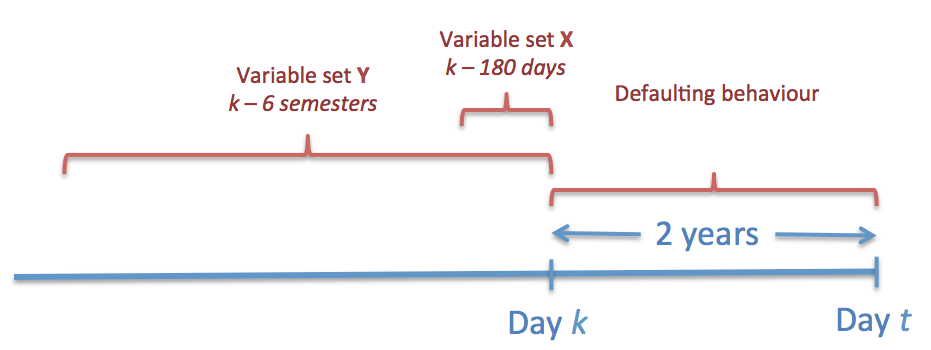
\includegraphics[scale=0.35]{figures/CajamarTimeLineReduced}
\caption{\label{fig:CajaMarTimeLineReduced}Time-line showing the generation of the data set. $t$ refers to the present time and $k$ corresponds to time $t-2$\ years. There are two disjoint groups of variables, denoted as $\X$ and $\Y$, with different past information considered, $180$ days back (daily) and $6$ semesters back (aggregated by semester), respectively.}
\end{figure}


The dataset is created at time $k$,  and contains a record for every client to be evaluated. 
Predictive variables refer here to the financial activity and payment behaviour of the customers in recent past as well as to their socio-demographic information which usually does not change over time. 

The  attributes denoted $\X$, for which financial activity  during the last 180 days is considered. Examples of these features include ``account balance'' and ``number of credit card operations''. 
These attributes usually change daily for a customer, so they are encoded by introducing a set of variables for each attribute, one for each day back from the current time $t$. 
Hence, the financial activity of a customer is specified by a number of variables equal to 180 times the number of attributes. 

For others attributes, denoted  $\Y$, we are interested in information from the last $36$ months. Examples of variables here include payments inside Cajamar (loans, mortgages, credits, etc.). 
The information from the last 36 months are grouped by semester, giving $6$ summary variables per attribute that is considered. 
Finally, there are some static variables (mainly includes socio-demographic variables) denoted by $\Z$. These are not included in \figref{CajaMarTimeLineReduced} as they are not time-indexed. 

The objective of the data analysis is to detect if a customer with profile $(\X,\Y,\Z)$ defaults within the next two years. This is determined by inspecting the user's behaviour from time $k$ and $2$ years into the future, i.e., in the period from $k$ to $t$ (see \figref{CajaMarTimeLineReduced}). We obtain this information directly from Cajamar's databases simply by selecting the time $k$ to be two back in time, and thereby letting $t$ be the current time. We use the variable \textit{Defaulter}. Note that, at the present time (time $t$), we have information of the \textit{Defaulter} variable in the period of time from $k$ to $t$. Thus,  Defaulter$^{(k)}$ indicates if at some point in this period the customer was a defaulter.

The full data set for training/updating the model is depicted in \tabref{TrainingDataset}. Each record contains the values for all predictive variables and a class variable. The class variable is labelled as \emph{non-defaulter} only when there is no defaulting in the period from $k$ to $t$ (2 years). 
\begin{table}[ht!]
\centering
\begin{tabular}{c|ccc|ccc|c|c}
	&\multicolumn{3}{c|}{Days} & \multicolumn{3}{c|}{Semester} & \\
     Time $t$              & $\X^{(k-180)}$ & $\ldots$ & $\X^{(k-1)} $ & $\Y^{(k-6)}$  & $\ldots$ & $\Y^{(k-1)} $ & $\Z$ & Defaulter$^{(k)}$\\  
\hline
Client$_1$  &                                                  &              &                     &                               &                     &        &  \\ 
$\vdots$      &                                                 &               &                     &                                &                     &       & \\ 
Client$_n$  &                                                &               &                     &                                &                     &     & \\ 
\end{tabular} 
\caption{Three groups of attributes $\X$, $\Y$ and $\Z$ are distinguished according to the past information required. Current time is denoted as $t$. The data set is built at time $t$ with $k=t - 2$ years. }
\label{tab:TrainingDataset} 
\end{table}

\subsubsection{The generated dataset}

The data set was generated at $t$ equal to December 31$^\text{st}$ 2013, thus simulating the calculations as if the AMIDST system was run two years before that ($k$ coresponds to December 31\textit{st} 2011). 
The dataset includes all customers who have been a client of Cajamar in the period  $k$ and up to day $t$, corresponding to $n=4.5\text{M}$ customers. 

Every member of the dataset has been classified as either non defaulter or defaulter (no missing entries). 
Customers can have missing attribute values in their description. In particular, some of the clients where not clients in the whole three year period before day $k$. If a customer was not associated to Cajamar at time $k - 6 \mbox{ semesters}$ e will not have direct access to the variables $\Y^{(k-6)}$. However, Cajamar will manually fill in all relevant missing values using other data sources.  Formally, every member $i$ of the dataset therefore has a vector of explanatory variables denoted by $\W_i=\{ \X_i^{(k-180)}, \ldots, \X_i^{(k-1)}, \Y_i^{(k-6)},\ldots, \Y_i^{(k-1)},\Z_i\}$ without missing values. In total, each customer is described using $7036$ variables.

Of all the customers in the dataset, $76\%$ are considered to be of no risk because they do not have a loan in the bank, approximately $20\%$ of the customers wee exposed but did not default, and $3.79\%$ of the customers  defaulted in the two-year period of interest. 

The data set will be used both for training and testing. The test-set is defined by randomly selecting $20\%$ of the customers. For reproducibility, a fixed random seed of  \comment{WHAT IS IT} was used to select the customers in the test set. 



\subsubsection{The models}

\comment{ SHOULD WE TAKE SOMETHING FROM D2.1 HERE, OR SKIP IT? I AM NOT SURE IF THE MODELS ARE OF RELEVANCE.}


\subsection{Predictive performance: test and evaluation}


\subsubsection{Application scenario 1}

The goal of the first application scenario is to determine if a customers is going to be a defaulters after two years. This corresponds to a classification problem, where the class variable is denoted Defaulter$^k$ in \tabref{TrainingDataset}. 

The approach of the AMIDST project is calculate $r_i=P(\mbox{Default}_i^k \,|\, \w_i)$ for each customer $i$. These quantities are afterwards update the risk table in the system (see Table~\ref{tab:riskTable}).
If, at some point, the probability of default of a customer rises above a predefined threshold, the bank may take preventive actions to reduce the risk of defaulting by this customer.

\begin{table}[ht!]
\centering
\begin{tabular}{c|ccc|ccc|c}
     Time $t$  & Risk of being defaulter \\  
\hline
Client$_1$  &    $r_1$  \\ 
$\vdots$      &   $\vdots$   \\ 
Client$_n$  &   $r_n$  \\ 
\end{tabular} 
\caption{Risk table for the bank customers where $r_i$ represents the probability of being defaulter for customer $i$.}
\label{tab:riskTable}
\end{table}



According to requirement CAJ.U3.D3, the risk prediction quality should be assessed using the area under the receiver operating characteristic (ROC) curve. 
The classification rule is that a customer $i$ is classified as a defaulter if $r_i \geq C$ for some constant $C$, and the ROC curve is computed by  plotting the rate of true positives against the rate of true negatives for various choices of $C$.  The requested area can then be found directly, and is according to the requirement to be larger than $0.90$. 

There are three main issues with the outlined approach:
\bde
\item[Relevance of the data:]  All the customers' data made available to the project for training and testing belong to people already associated with Cajamar, and their economic status (e.g., regarding whether or not they have obtained a loan) is a consequence of Cajamar's current system being employed to remove the customers not deemed appropriate. The dataset we have access to may therefore not reflect the distribution of customers that approach Cajamar in the first place (and which AMIDST will be exposed to if employed in production).

\item[Changes in the economic climate:]  A Cajamar customer's chance of defaulting is to some  extent determined by external factors, like the economic climate in Spain. During the economic crises the rate of defaulters was significantly higher than what was observed prior to the onset of the crisis. The data set we work with is from the period of the crisis, and it is natural to expect that the relationships found by the model are optimized for that economic climate. The AUC criteria is chosen to remedy global effects that affect all customers in a similar way, but we can still not guarantee that the model will perform at a similar level for fundamentally different economic climate.

\item[Stable versus volatile climate:] Customers in the training and test sets are per definition from the same time period. Learning from the training data, we will therefore be able to detect the economic climate to which the customers will be exposed (e.g., simply by detecting the fraction of defaulters in the training data). If put in production, the predictions AMIDST are asked to make will be about the future, i.e., shifted two years in time when compared to the training data. This is not a problem if the economic climate is static or only slowly varying, but will be disastrous if, for instance, AMIDST is asked to make predictions about future customers immediately before the outset of a new economic crisis.

\ede

To partly account for these shortcomings of the test procedure we have collected another dataset with $k$ equal to December 31st 2013, and where the correct class labels will be discovered two years later (December 31st 2015). 
An AUC of more than $90\%$ when using this new dataset for testing (and the original dataset for training) would be seen as a strong indication of the applicability of AMIDST in production.

\comment{Remove this part, or will we have the extra data? I am writing that the data has already been generated just to comply with the ``Data available from Day 1''-requirement from our friends in EU.}






\subsubsection{Application scenario 2}




A marketing campaign in Cajamar involves two steps.  The first step is conducted by the marketing department, and results in a list of candidate customers. 
The list contains clients that have a high probability of signing what is offered (for instance a credit card).  The second step, conducted by the risk modellers, is to filter out clients that are risky in terms of defaulting.
The task described in Use case 4 is to find relevant users profiles to conduct marketing campaigns. The profiles should contain customers that are like to be non-defaulters, and cover only attributes that are found to be relevant by the domain experts. It is required (CA.U6.O3) that the expected benefits of a marketing campaign using obtained profiles should be $5\%$ higher than with current methods. 

Direct quantitative evaluation of the AMIDST-generated profiles is difficult to perform in a formal way. The first issue is that the application scenarios generates \textit{user profiles} and not \textit{set of user}. 
We cannot value a profile in itself; it is the application of the profile to generate user sets that potentially can be monetized. The second problem is that the AMIDST profile defines users that are not likely to default, not users that are likely to contract (and therefore not necessarily users who are valuable as marketing objects). For instance, it seems natural to expect the AMIDST profile to prefer solvent customers living in their own homes without any mortgage and with a sizable cash-account. On the other hand, a customer like that may not be relevant to target for a campaign selling small-sized cash-loans without security requirements. We therefore propose that the project extraction is evaluated qualitatively as follows:

\bit
\item A historical marketing campaign is selected, and the set of customers contacted are listed. The set of customers is called $\calC$.
\item The AMIDST system is used to generate a profile for non-defaulting customers, and a fixed number of  customers fitting the profile (comparable to the number of elements in $\calC$) are selected.
\item The marketing department selects a subset of the customers in this set based on their probability to contract. Call this reduced set of customers $\calA$.
\item The two sets $\calC$ and $\calA$ are compared qualitatively.
\eit

To target the quantitative requirement, we also propose to utilize the AMIDST risk prediction capability from application scenario 1 in the marketing setting, where the following procedure will be performed:
\bit
\item Select a historical marketing campaign that is at least two years old. The set of customers is called $\calC$.
\item Obtain the empirical risk of the campaign during the two year period (see Section XX). \comment{Sigve will write about empirical loss etc in another part of the overall document.} 
\item  Filter clients that the AMIDST system deems too risky. The set of customers is called $\calA$. Note that $\calA\subseteq\calC$.
\item Calculate the empirical risk of the set $\calA$. The risk of $\calA$ should be at least $5\%$ lower than the risk of the set $\calC$.
\eit
It should be noted that this procedure only evaluates the AMIDST system's ability to remove poor customers from the list of customers that were included in the campaign, and we are not able to determine the effect of AMIDST potentially wanting to send marketing material to customers that were not selected for the historical campaign. 


\comment{From Ramon:

\bit
\item Another thing that can be done is to estimate the benefit of clients that AMIDST would have included (using expected income and expected loss) and add it to the benefit of the virtual AMIDST campaign.
\eit

Should we add that?}




\comment{Rest of the section is Sigve's text. I propose that we remove all the math into the start-up-sections and just use established stuff like ``Empirical risk'' here. Not sure if all of Sigve's points have been included in the ``for dummies'' - version I have written. Must be checked.}



There are more opportunities with testing the second step.  After performing step one the test data set is reduced to a set of clients with a high contracting probability (i.e. above a certain level).  Let the clients in this data set be $(x_i, y_i)$, where $y_i$ is either default or not default and $x_i$ is a vector of explanatory variables.  It makes sense to compute AUC for both the current method and the Amidst method to compare the two methods.  This comparison will say something about the ability of the filter to take out defaulters, while keeping the non defaulters.  However, we must assume that the real probability of contracting $P(\bv{x_i})$ is completely independent of whether the client will actually default or not.

Moreover, in Delivery 1.2, it is required that the benefit of a AMIDST induced marketing campaign should be more than 5 percent higher than a normal campaign.  In order to discuss such a requirement we have to iintroduce a function that describes the financial loss of a certain classification rule compared to a classification rule that make no mistakes. 

In this paper, we define the \emph{loss function} as a real and lower-bounded function $L(x_i, h(x_i), y_i)$. It takes into account the explanatory variables for each client $x_i$, the predicted class $h(x_i)$ and the true class label $y_i$. 

In the current system in Cajamar the classification rule is denoted $h_{\mbox{Current},L_1}$ and is defined by

\begin{equation}
\label{def:empRisk}
h_{\mbox{Current},L_1}(x_i) = P_{\mbox{Current}}(\mbox{Default}_i \,|\, \bv{x_i}) \leq L_1 
\end{equation}
where the probability for defaulting client $i$ are $P_{\mbox{Current}}(\mbox{Default}_i \,|\, \bv{x_i})$.  Here, $L_1$ is a chosen classification limit. 

We let the cost of excluding client $i$ that does not default as $c_i(0|1)$ and also the cost of including client $i$ that does default as $c_i(1|0)$.  Both costs are related to the size of the potential offer.  Also, we make the assumption that the real probability of contracting $P(\bv{x_i}) = p$ is completely independent of whether the client will actually default or not.  The loss function below is of interest

\begin{equation}
\label{def:empRiskBank}
L(x_i, h_{\mbox{Current},L_1}(x_i) , y_i) = 
\begin{cases}
0     &\quad \mbox{for} \quad h_{\mbox{Current},L_1}(x_i) = 0 \quad \& \quad y_i = 0\\
p c_i(1|0)    &\quad \mbox{for} \quad h_{\mbox{Current},L_1}(x_i) = 1 \quad \& \quad y_i = 0\\
p c_i(0|1)      &\quad \mbox{for} \quad h_{\mbox{Current},L_1}(x_i) = 0 \quad \& \quad y_i = 1\\
0   &\quad \mbox{for} \quad h_{\mbox{Current},L_1}(x_i) = 1 \quad \& \quad y_i = 1.
\end{cases}
\end{equation}
Notice that $L$ is an array of $n \times 2\times 2$ elements. Cajamar can estimate $c_i(0|1)$ and $c_i(1|0)$ for all clients in the database.

The empirical risk is found by averaging the loss function on the training set given by 

\begin{equation}
\label{def:empRisk}
R_{emp}(h_{\mbox{Current},L_1}, \bv{x}) = n^{-1} \sum_{i=1}^n L(x_i, h_{\mbox{Current},L_1}(x_i), y_i).
\end{equation}

It is now possible to calculate the empirical risk involved with using both the current filter and also the Amidst filter.  It is therefore possible to estimate the ratio between the costs and therefore see whether there is more than 5 percent gain in using the Amidst default filter compared to using the current default filter.  Notice that in terms of estimating this gain percentage it is not needed to estimate $p$.  However, it could be estimated from the number that accepted the offer on an old campaign.


\subsubsection*{Calculating empirical risk on an old campaign}

It is also possible to use an old campaign to test the improvement of using the Amidst default filter in addition to the current filter. 

Consider an old campaign that was done more than two years ago. Even though costs and default/non defaults are known for all clients, the loss function is only known on the clients that was targeted in that campaign.  This makes this discussion complicated. 

We will now consider the AMIDST induced marketing campaign as a binary classification problem with class variable $y_i$, which can take the values $\{0,1\}$. Class one refers to non-defaulters that actually signs the contract and class zero refers to the rest of the clients.  In a perfect campaign only the non-defaulters that actually signs the offer (for instance a credit card or a loan) are selected.  

In the current system in Cajamar the classification rule is denoted $h_{\mbox{Current},L_1,L_2}$ and is defined by

\begin{equation}
\label{def:empRisk}
h_{\mbox{Current},L_1,L_2}(x_i) = P_{\mbox{Current}}(\mbox{Default}_i \,|\, \bv{x_i}) \leq L_1 \, \& \,P_{\mbox{Current}}(\mbox{Contract}_i \,|\, \bv{x_i}) \geq L_2,
\end{equation}
where the probability for defaulting and contracting for client $i$ are $P_{\mbox{Current}}(\mbox{Default}_i \,|\, \bv{x_i})$ and $P_{\mbox{Current}}(\mbox{Contract}_i \,|\, \bv{x_i})$.  Here, $L_1$ and $L_2$ are chosen classification limits. 

We let the cost of excluding client $i$ that actually would contract and not default as $c_i(0|1)$.  This cost is related to the size of the potential offer.

Moreover, we let $c_i(1|0)$ be the cost of offering to client $i$, provided that he either would not take the offer or would default if he took the offer.  Clearly, if client $i$ was offered and contracted but defaulted, $c_i(1|0)$ is related to the size of the contract.  Otherwise, $c_i(1|0)$ is only related to the cost of making the offer.  The loss function below is of interest

\begin{equation}
\label{def:empRiskBank}
L(x_i, h_{\mbox{Current},L_1,L_2}(x_i) , y_i) = 
\begin{cases}
0     &\quad \mbox{for} \quad h_{\mbox{Current},L_1,L_2}(x_i) = 0 \quad \& \quad y_i = 0\\
c_i(1|0)    &\quad \mbox{for} \quad h_{\mbox{Current},L_1,L_2}(x_i) = 1 \quad \& \quad y_i = 0\\
c_i(0|1)      &\quad \mbox{for} \quad h_{\mbox{Current},L_1,L_2}(x_i) = 0 \quad \& \quad y_i = 1\\
0   &\quad \mbox{for} \quad h_{\mbox{Current},L_1,L_2}(x_i) = 1 \quad \& \quad y_i = 1.
\end{cases}
\end{equation}

Cajamar can estimate $c_i(0|1)$ and $c_i(1|0)$ for all clients in the database.


The empirical risk for the old campaign is not taking into account the financial loss related to excluding a number of clients that actually would have contracted and not defaulted.  Said with other words, the empirical risk is not taking into account losses related to when $h_{\mbox{Current},L_1,L_2}(x_i) = 0$, and $y_1 = 1$.  In such a calculation none of the $c_i(0|1)$s are used.  The empirical risk will therefore be less than the true risk (which would take the above point into account).

A simple test is to use the Amidst toolbox to provide an additional filter related to default prediction on top of the old classification rule.  Mathematically this is

\begin{equation}
\begin{split}
\label{eq:filter}
h_{\mbox{Amidst filter},L_1,L_2,L_3}(x_i) = &
P_{\mbox{Current}}(\mbox{Default}_i \,|\, \bv{x_i}) \leq L_1
 \, \& \,
P_{\mbox{Current}}(\mbox{Contract}_i \,|\, \bv{x_i}) \geq L_2
\, \& \,  
\\ &
P_{\mbox{Amidst filter}}(\mbox{Default}_i \,|\, \bv{x_i}) \leq L_3.
\end{split}
\end{equation}
This calculation of empirical risk is biased by the same amount as the old method.  It makes therefore sense to compare $R_{emp}(h_{\mbox{Amidst filter},L_1,L_2,L_3}, \bv{x}) $ with $R_{emp}(h_{\mbox{Current},L_1,L_2}, \bv{x}) $.
The benefit of using the Amidst model as additional filter can therefore be quantified.

\subsection*{Questions: }
\begin{enumerate}
\item Do you see any flaw in reasoning?
\item What more should we do?
\item What do you think about the profiling ideas?
\end{enumerate}




\subsection{Run-time performance: test and evaluation}
\subsubsection{Application scenario 1}

According to the requirement procedure, the full process starting with SQL statements and ending with validation of the new risks should be complicated in no more than three hours (CAJ.U1.O1, CAJ.U2.O1, CAJ.U4.D1, CAJ.U5.O1).


\comment{Testing procedure/how strictly we will look at this must be evaluated.}

\comment{Mention the hardware specified in R1.2, p. 9?}


\subsubsection{Application scenario 2}

There are no specific run-time requirements for this application scenario. Specifically, it is stated that \textit{``[\ldots] execution time of this process is not relevant because the marketing campaigns are not launched so frequently.''}.



\vekk{

\newpage




%% This part written by Sigve. I'm keeping it here for reference (and copy-paste'ing. Rewrite to conform with the new layout of the document. 
%% This work initiated by Helge Langseth on Nov 20th 2014

There are two application scenarios here.  The first one is prediction of whether a client will default within two years or not and the second is related to the benefit of a marketing campaign. For clarity we have added the description about the data set from delivery 2.1 without any modification.

\section{Description from 2.1}

%-------------------------------------------------------------------------------------------------------
\subsection{Predicting probability of default} \label{SubSection:Predicting}
%-------------------------------------------------------------------------------------------------------

Our objective is to tackle the current limitations of the risk prediction problem by \textit{daily} learning the predictive model and also updating the risk of default for every bank customer. Dependences among the variables will now be considered, as well as including all the variables in the analysis. With these changes, Cajamar plans to improve the quality of the prediction model by increasing the area under ROC curve significantly.


Therefore, the process will consist in building a \textit{training set} as well as a set of customers to be evaluated, called \textit{evaluation set} (see Deliverable 1.2~\cite{Fer14b}). How these data sets are generated gives us some insights into the nature of this risk prediction problem (see Figure~\ref{Figure:CajaMarTimeLine} for a better understanding):

%Next, we detail how these data sets are collected .
%Figure~\ref{Figure:CajaMarTimeLine} illustrates how both evaluation and training data sets are collected within a time-line. The current time is denoted as $t$ and the time $2$ years back as $k$, i.e., $k=t-2$ years. 

\begin{figure}[ht!]
\centering
\includegraphics[scale=0.35]{figures/CajamarTimeLine}
\caption{\label{Figure:CajaMarTimeLine}Time-line showing the generation of the evaluation (in green) and training (in red) data sets. $t$ refers to the present time and $k$ corresponds to time $t-2$\ years. Both in the training and test data sets, there are two disjoint groups of variables, denoted as $\X$ and $\Y$, with different past information considered, $180$ days back (daily) and $6$ semesters back (by semester), respectively.}

\end{figure}

\begin{itemize}

\item \textbf{Model evaluation data set:} This data is created at time $t$ and contains a record for every client to be evaluated. Note that information about the predicted defaulting behaviour is missing at time $t$ and it will be obtained after performing inference on the model. Predictive variables refer here to the financial activity and payment behaviour of the customers in recent past as well as to their socio-demographic information which usually does not change over time. 

There are attributes, denoted as $\X$, for which information during the last 180 days is considered. 
%recent \textcolor{red}{{\bf financial activity}}of a customer refers to attributes such as ``account balance'', ``number of credit card operations'', etc. stored in the last 180 days. 
These attributes usually change daily for a customer, so they are encoded by introducing a set of variables for each attribute, one for each day back from the current time $t$. Hence, the financial activity of a customer is specified by a number of variables equal to 180 times the number of attributes. For others attributes, denoted as $\Y$, we are interested in information from the last $36$ months grouped by semester. 
%In the case of \textcolor{red}{{\bf past payment behaviour}}, the attributes refer to variables related to \textcolor{red}{payments inside Cajamar (loans, mortgages, credits, etc.).} Information from the last 36 months grouped by semester is considered for these variables. 
Therefore, similar to previous group of variables, $6$ variables for each of these attributes will be considered. Finally, there are some other static variables, denoted as $\Z$, not included in Figure~\ref{Figure:CajaMarTimeLine} as they are not indexed over time. The data set for the evaluation of customers is depicted in Table~\ref{tab:EvaluationDataset}. 


%with information about \textcolor{red}{payments to other financial institutions or companies (phone and electricity bills, public bodies, etc.)} 
%are included in this group of variables. They are denoted as .

%The group of variables denoted as $\Z$ mainly includes socio-demographic variables and they are not indexed over time as they remain fixed.  

\begin{table}[ht!]
\centering
\begin{tabular}{c|ccc|ccc|c}
	&\multicolumn{3}{c|}{Days} & \multicolumn{3}{c|}{Semester} \\
     Time $t$              & $\X^{(t-180)}$ & $\ldots$ & $\X^{(t-1)} $ & $\Y^{(t-6)}$  & $\ldots$ & $\Y^{(t-1)} $ & $\Z$  \\  
\hline
Client$_1$  &                                                  &              &                     &                               &                     &        \\ 
$\vdots$      &                                                 &               &                     &                                &                     &      \\ 
Client$_n$  &                                                &               &                     &                                &                     &     \\ 
\end{tabular}
\caption{Evaluation data set at time $t$ for all the clients. Three groups of attributes $\X$, $\Y$ and $\Z$ are distinguished according to the past information required. Current time is denoted as $t$.}
\label{tab:EvaluationDataset} 
\end{table}

Thus, the objective is to compute the probability of defaulting within the following two years of each record from the evaluation data set, and afterwards update the risk table in the system (see Table~\ref{tab:riskTable}).

\begin{table}[ht!]
\centering
\begin{tabular}{c|ccc|ccc|c}
     Time $t$  & Risk of being defaulter \\  
\hline
Client$_1$  &    $r_1$  \\ 
$\vdots$      &   $\vdots$   \\ 
Client$_n$  &   $r_n$  \\ 
\end{tabular} 
\caption{Risk table for the bank customers where $r_i$ represents the probability of being defaulter for customer $i$.}
\label{tab:riskTable}
\end{table}

If, at some point, the probability of default of a customer rises above a predefined threshold, the bank may take preventive actions to reduce the risk of defaulting by this customer.


\item \textbf{Model training data set:}  This data set is also built at time $t$ in a similar way as the evaluation data. It contains the same set of features as well as the target variable \textit{Defaulter} but with information referred to time $k$ instead (two years back). Note that, at time $t$, we have information of the \textit{Defaulter} variable in the period of time from $k$ to $t$. Thus,  Defaulter$^{(k)}$ indicates if at some point in this period she/he was a defaulter.

The data set for training/updating the model is depicted in Table~\ref{tab:TrainingDataset}.
\begin{table}[ht!]
\centering
\begin{tabular}{c|ccc|ccc|c|c}
	&\multicolumn{3}{c|}{Days} & \multicolumn{3}{c|}{Semester} & \\
     Time $t$              & $\X^{(k-180)}$ & $\ldots$ & $\X^{(k-1)} $ & $\Y^{(k-6)}$  & $\ldots$ & $\Y^{(k-1)} $ & $\Z$ & Defaulter$^{(k)}$\\  
\hline
Client$_1$  &                                                  &              &                     &                               &                     &        &  \\ 
$\vdots$      &                                                 &               &                     &                                &                     &       & \\ 
Client$_n$  &                                                &               &                     &                                &                     &     & \\ 
\end{tabular} 
\caption{Training data set built at time $t$ with $k=t - 2$ years.  The notation for predictive variables is the same as in Table~\ref{tab:EvaluationDataset}.}
\label{tab:TrainingDataset} 
\end{table}

Table~\ref{tab:TrainingDataset} shows the training data set where each record contains the values for all predictive variables and a class value labelled as \emph{non-defaulter} only when there is no evidence of defaulting in the period from $k$ to $t$ (2 years). 

\end{itemize}

\section{Test and evaluation regime}

The training set above is actually the data set that we are going to train on and also test on. This may be a source to confusion, but from now on the training set above will be defined as the dataset and the evaluation set is not even considered in relation to testing. 

The only criterion for being a member of the dataset is that the member has been a client continuously from day $k$ and up to day $t$.  Every member of the dataset has a class label that is either non defaulter or defaulter.  There are no missing values related to class labels.  However, there are missing values related to attributes.  In particular, some of the clients where not clients in the whole three year period before day $k$.  Cajamar will manually fill in all relevant missing values.  Formally, every member $i$ of the dataset has a vector of explanatory variables that is denoted by $\bv{x_i} =\{ \X_i^{(k-180)},  \X_i^{(k-1)}, ...\Y_i^{(k-6)}, \Y_i^{(k-1)},\Z_i\}$.  

We will divide this data set into a training set and a test set by a completely random process.

\subsection{Requirements for the first use case scenario: default prediction}

In the first use case scenario, it is required that the AUROC should be above 0.90.
 
The Bayesian network basically computes the probability $P(\mbox{Default}_i \,|\, \bv{x_i})$ and the classification rule is
$P(\mbox{Default}_i \,|\, \bv{x_i}) \geq C$.  The ROC curve is computed by basically plotting the rate of true positives against the rate of true negatives for various choices of $C$.  AUROC is the area under the graph.  (There is also another way of computing AUROC which do not involve computing the rate of true positives and rate true negatives for various $C$, but this is omitted in this discussion.)

\subsubsection*{Questions: }
\begin{enumerate}
\item How many defaulters and non defaulters do we have on both the training set and the test set?
\item Can you go though all the information and make sure that it is correct.
\end{enumerate}


\subsection{Requirements for the second use case scenario:  AMIDST induced marketing campaign}

A marketing campaign in Cajamar involves two steps.  The first step is to find clients that have a high probability of signing what is offered (for instance a credit card).  The second step is to filter out clients that are risky in terms of defaulting.
The testing regime involves testing each step separately.

The first step is difficult to test. We suggest that the Amidst profiler finds a list of a certain number of clients that are manually inspected by the marketing department in Cajamar. This list can for instance be compared to a list of clients with high contracting probability from a former campaign.

There are more opportunities with testing the second step.  After performing step one the test data set is reduced to a set of clients with a high contracting probability (i.e. above a certain level).  Let the clients in this data set be $(x_i, y_i)$, where $y_i$ is either default or not default and $x_i$ is a vector of explanatory variables.  It makes sense to compute AUC for both the current method and the Amidst method to compare the two methods.  This comparison will say something about the ability of the filter to take out defaulters, while keeping the non defaulters.  However, we must assume that the real probability of contracting $P(\bv{x_i})$ is completely independent of whether the client will actually default or not.

Moreover, in Delivery 1.2, it is required that the benefit of a AMIDST induced marketing campaign should be more than 5 percent higher than a normal campaign.  In order to discuss such a requirement we have to iintroduce a function that describes the financial loss of a certain classification rule compared to a classification rule that make no mistakes. 

In this paper, we define the \emph{loss function} as a real and lower-bounded function $L(x_i, h(x_i), y_i)$. It takes into account the explanatory variables for each client $x_i$, the predicted class $h(x_i)$ and the true class label $y_i$. 

In the current system in Cajamar the classification rule is denoted $h_{\mbox{Current},L_1}$ and is defined by

\begin{equation}
\label{def:empRisk}
h_{\mbox{Current},L_1}(x_i) = P_{\mbox{Current}}(\mbox{Default}_i \,|\, \bv{x_i}) \leq L_1 
\end{equation}
where the probability for defaulting client $i$ are $P_{\mbox{Current}}(\mbox{Default}_i \,|\, \bv{x_i})$.  Here, $L_1$ is a chosen classification limit. 

We let the cost of excluding client $i$ that does not default as $c_i(0|1)$ and also the cost of including client $i$ that does default as $c_i(1|0)$.  Both costs are related to the size of the potential offer.  Also, we make the assumption that the real probability of contracting $P(\bv{x_i}) = p$ is completely independent of whether the client will actually default or not.  The loss function below is of interest

\begin{equation}
\label{def:empRiskBank}
L(x_i, h_{\mbox{Current},L_1}(x_i) , y_i) = 
\begin{cases}
0     &\quad \mbox{for} \quad h_{\mbox{Current},L_1}(x_i) = 0 \quad \& \quad y_i = 0\\
p c_i(1|0)    &\quad \mbox{for} \quad h_{\mbox{Current},L_1}(x_i) = 1 \quad \& \quad y_i = 0\\
p c_i(0|1)      &\quad \mbox{for} \quad h_{\mbox{Current},L_1}(x_i) = 0 \quad \& \quad y_i = 1\\
0   &\quad \mbox{for} \quad h_{\mbox{Current},L_1}(x_i) = 1 \quad \& \quad y_i = 1.
\end{cases}
\end{equation}
Notice that $L$ is an array of $n \times 2\times 2$ elements. Cajamar can estimate $c_i(0|1)$ and $c_i(1|0)$ for all clients in the database.

The empirical risk is found by averaging the loss function on the training set given by 

\begin{equation}
\label{def:empRisk}
R_{emp}(h_{\mbox{Current},L_1}, \bv{x}) = n^{-1} \sum_{i=1}^n L(x_i, h_{\mbox{Current},L_1}(x_i), y_i).
\end{equation}

It is now possible to calculate the empirical risk involved with using both the current filter and also the Amidst filter.  It is therefore possible to estimate the ratio between the costs and therefore see whether there is more than 5 percent gain in using the Amidst default filter compared to using the current default filter.  Notice that in terms of estimating this gain percentage it is not needed to estimate $p$.  However, it could be estimated from the number that accepted the offer on an old campaign.


\subsubsection*{Calculating empirical risk on an old campaign}

It is also possible to use an old campaign to test the improvement of using the Amidst default filter in addition to the current filter. 

Consider an old campaign that was done more than two years ago. Even though costs and default/non defaults are known for all clients, the loss function is only known on the clients that was targeted in that campaign.  This makes this discussion complicated. 

We will now consider the AMIDST induced marketing campaign as a binary classification problem with class variable $y_i$, which can take the values $\{0,1\}$. Class one refers to non-defaulters that actually signs the contract and class zero refers to the rest of the clients.  In a perfect campaign only the non-defaulters that actually signs the offer (for instance a credit card or a loan) are selected.  

In the current system in Cajamar the classification rule is denoted $h_{\mbox{Current},L_1,L_2}$ and is defined by

\begin{equation}
\label{def:empRisk}
h_{\mbox{Current},L_1,L_2}(x_i) = P_{\mbox{Current}}(\mbox{Default}_i \,|\, \bv{x_i}) \leq L_1 \, \& \,P_{\mbox{Current}}(\mbox{Contract}_i \,|\, \bv{x_i}) \geq L_2,
\end{equation}
where the probability for defaulting and contracting for client $i$ are $P_{\mbox{Current}}(\mbox{Default}_i \,|\, \bv{x_i})$ and $P_{\mbox{Current}}(\mbox{Contract}_i \,|\, \bv{x_i})$.  Here, $L_1$ and $L_2$ are chosen classification limits. 

We let the cost of excluding client $i$ that actually would contract and not default as $c_i(0|1)$.  This cost is related to the size of the potential offer.

Moreover, we let $c_i(1|0)$ be the cost of offering to client $i$, provided that he either would not take the offer or would default if he took the offer.  Clearly, if client $i$ was offered and contracted but defaulted, $c_i(1|0)$ is related to the size of the contract.  Otherwise, $c_i(1|0)$ is only related to the cost of making the offer.  The loss function below is of interest

\begin{equation}
\label{def:empRiskBank}
L(x_i, h_{\mbox{Current},L_1,L_2}(x_i) , y_i) = 
\begin{cases}
0     &\quad \mbox{for} \quad h_{\mbox{Current},L_1,L_2}(x_i) = 0 \quad \& \quad y_i = 0\\
c_i(1|0)    &\quad \mbox{for} \quad h_{\mbox{Current},L_1,L_2}(x_i) = 1 \quad \& \quad y_i = 0\\
c_i(0|1)      &\quad \mbox{for} \quad h_{\mbox{Current},L_1,L_2}(x_i) = 0 \quad \& \quad y_i = 1\\
0   &\quad \mbox{for} \quad h_{\mbox{Current},L_1,L_2}(x_i) = 1 \quad \& \quad y_i = 1.
\end{cases}
\end{equation}

Cajamar can estimate $c_i(0|1)$ and $c_i(1|0)$ for all clients in the database.


The empirical risk for the old campaign is not taking into account the financial loss related to excluding a number of clients that actually would have contracted and not defaulted.  Said with other words, the empirical risk is not taking into account losses related to when $h_{\mbox{Current},L_1,L_2}(x_i) = 0$, and $y_1 = 1$.  In such a calculation none of the $c_i(0|1)$s are used.  The empirical risk will therefore be less than the true risk (which would take the above point into account).

A simple test is to use the Amidst toolbox to provide an additional filter related to default prediction on top of the old classification rule.  Mathematically this is

\begin{equation}
\begin{split}
\label{eq:filter}
h_{\mbox{Amidst filter},L_1,L_2,L_3}(x_i) = &
P_{\mbox{Current}}(\mbox{Default}_i \,|\, \bv{x_i}) \leq L_1
 \, \& \,
P_{\mbox{Current}}(\mbox{Contract}_i \,|\, \bv{x_i}) \geq L_2
\, \& \,  
\\ &
P_{\mbox{Amidst filter}}(\mbox{Default}_i \,|\, \bv{x_i}) \leq L_3.
\end{split}
\end{equation}
This calculation of empirical risk is biased by the same amount as the old method.  It makes therefore sense to compare $R_{emp}(h_{\mbox{Amidst filter},L_1,L_2,L_3}, \bv{x}) $ with $R_{emp}(h_{\mbox{Current},L_1,L_2}, \bv{x}) $.
The benefit of using the Amidst model as additional filter can therefore be quantified.

\subsection*{Questions: }
\begin{enumerate}
\item Do you see any flaw in reasoning?
\item What more should we do?
\item What do you think about the profiling ideas?
\end{enumerate}

}



\bibliographystyle{named}
\bibliography{ijcai13}

\end{document}



\section{Daimler: test and evaluation}




% !TEX TS-program = pdflatex
\documentclass{article}

\usepackage{hl_short}
\usepackage{times}
\usepackage{graphicx}
\usepackage{latexsym}

\usepackage{bm}
\usepackage{amsbsy}
\usepackage{amsmath}
\usepackage{amsfonts}
\usepackage{amssymb}

\usepackage{subfigure}
\usepackage{color}

\usepackage{theorem}

\theoremstyle{theorem}
\newtheorem{theorem}{Theorem}

\usepackage{array}

\theoremstyle{definition}
\newtheorem{definition}{Definition}
\newtheorem{remark}{Remark}

\newcommand{\bu}[1]{\mathbf{#1}}
\newcommand{\bv}[1]{\bm{#1}}


\newcommand{\W}{\mathbf{W}}
\newcommand{\X}{\mathbf{X}}
\newcommand{\Y}{\mathbf{Y}}
\newcommand{\Z}{\mathbf{Z}}
\newcommand{\w}{\mathbf{w}}
\newcommand{\x}{\mathbf{x}}
\newcommand{\y}{\mathbf{y}}
\newcommand{\z}{\mathbf{z}}
\newcommand{\argmax}[1]{\underset{#1}{\operatorname{arg}\,\operatorname{max}}\;}

\newcommand{\comment}[1]{ \begin{center}{\bf [[ #1 ]]}\end{center}}

\title{Practical Considerations for Testing the Verdande Technology Use Case}
%\author{Sigve, Helge, Thomas}
\date{\today}


\begin{document}
\maketitle


\section{Verdande Technology: Test and evaluation}



\subsection{Use-case requirements}

The test and evaluation procedures for Verdande Technology will be developed along the lines introduced in Deliverable 2.1: Instead of testing each use case separately, we utilize the notion of {\em application scenarios}. 
An application scenario is defined by a sequence of use cases that combined constitutes a full interaction procedure leading to a verifiable result. In D2.1 we defined two scenarios:

\begin{itemize}
\item VER1: 
Detection of drill string vibrations:
The application scenario covers these use cases from (D1.2):
\begin{itemize}
\item UC1: Parsing data sets
\item UC2: Erratic torque detection (model construction)
\item UC5: Model application
\item UC6: Result generation
\end{itemize}

\item VER2: Semi-automatic labelling:
The application scenario covers these use cases from (D1.2):
\begin{itemize}
\item UC1: Parsing data sets
\item UC3: Semi-automatic labelling (model construction)
\item UC5: Model application
\item UC6: Result generation
\end{itemize}

\item VER3: Automatic formation detection:
The application scenario covers these use cases from (D1.2):
\begin{itemize}
\item UC1: Parsing data sets
\item UC4: Formation detection (model construction)
\item UC5: Model application
\item UC6: Result generation
\end{itemize}

\end{itemize}

Requirements for the different use-cases were defined in D1.2. Most requirements are functional in nature, and introduce functionality requests into the system, but some also introduce hard requirements that can be tested quantitatively. The latter are repeated in \ref{tab:verdande:requirements} for completeness. We note that the requirements centers around three issues:
\begin{itemize}
\item The whole process covered by Application scenario CAJ1, starting with SQL queries and ending with report generation must take less than 3 hours for the 5.6M clients (requirements CAJ.U1.O1, CAJ.U2.O1, CAJ.U4.D1, CAJ.U4.O1, and CAJ.U5.O1).
\item The prediction quality for Application scenario CAJ1, evaluated by AUROC, must be higher than $90\%$ (CAJ.U3.D3).
\item The quality of the profiles generated in Application scenario CAJ2 are evaluated through an improved benefit of at least $5\%$ (CAJ.U6.O3).
\end{itemize}

\begin{table}
\scalebox{.89}{

\begin{tabular}{|p{16mm}|p{15mm}|p{75mm}|p{12mm}|}\hline
ID & Sub-phase & Description & Task(s)\\ \hline\hline
VER.U1.O1&	Software development	&Data import should take less than 10 minutes  on a single desktop computer or equivalent	&	7.1\\ \hline
VER.U2.O2& 	Production testing	& Formalization of the test procedure will be developed in task 1.2. & 1,2 /\, 7.2\\ \hline
VER.U2.D3&	Production testing	& The accuracy of the result and the discussion should be published in a journal or a conference.  & 7.2 /\, 9.3 /\, 9.4\\\hline
VER.U3.O2& 	Production testing	& The rate of missed abnormalities must be no larger than the prior probability of abnormality.  &  7.2\\ \hline
VER.U3.D3&	Production testing	&The rate of missed normal states must be no larger than the prior probability of normality.  & 7.2\\\hline
VER.U3.O4& 	Production testing	& The rate of missed abnormalities could be below what is obtained by an inexperienced drilling engineer or a software program at that level. & 7.2\\ \hline
VER.U3.D5&	Production testing	& The rate of missed normalities could be below what is obtained by an inexperienced drilling engineer or a software program at that level.  & 7.2\\\hline
VER.U4.O2& 	Production testing	& MD algorithm must be less than MD prior (both defined in Use Case Scenario 3), on at least 1 randomly chosen drilling log.  &  7.3\\ \hline
VER.U4.D3&	Production testing	&MD algorithm should be 10 percent less than MD prior, defined in Use Case Scenario 2, on at least 3 randomly chosen drilling logs.  & 7.3\\\hline
VER.U5.D4&	Testing	& Agents need to run fast enough for real-time implementation. In practice, this means that once probability tables are calculated  (post learning), the agent once provided a single new data point must be able to calculate probabilities, values or classifications and returning these in under 1 second on a single desktop computer or equivalent hardware  & 3.3 / 7.3\\\hline
\\
\hline \hline\end{tabular}

}
\caption{Testable requirements for the Verdande use-cases. }\label{tab:verdande:requirements}
\end{table}

\subsection{Model and data characteristics}

%\comment{The following is from D2.1}
In order to make this document self contained, the summary of the Verdande Technology use case scenarios are repeated below.

\begin{enumerate}
\item {\bf Automatic detection of drill string vibrations and abnormal torque
states} This task aims to better diagnose the shape of the wellbore and the
state of the equipment, make better decisions on how to manage the well, and
thereby reduce the non-productive time. Currently, the state-of-the-art algorithm
in DrillEdge is based on detecting erratic torque. It is a simple algorithm
based on comparing root mean squared differences in a time window between the
measured torque and a smoothed version of the torque. In essence, this method is
measuring the local amplitude variations in the torque. Additionally, the algorithm
is altering out abnormal torque during connections and some other instances. This
simple algorithm is rather limited and does not inherently take into account the
existing uncertainty in the streaming data. The main objective for this scenario
is then to design a probabilistic graphical model for erratic torque monitoring and
detection of abnormal situations.
\item {\bf Semi-automatic labelling} The main contribution from DrillEdge [28] during
operation is that it enables the driller to see in real time if the current situation
is \emph{ similar} to previous situations that lead to undesired circumstances. If this
is the case, remedial actions can be found to avoid undesired events. At the
core of the analysis are historical examples of noteworthy episodes, ranging from
clearly undesired events, for instance getting stuck, to more subtle indications of
evolving problems, such as abnormal readings of hook-load. Verdande Technology
has already extensive datasets, where such episodes are identified. However, the
denitions of the episodes are not always crisp, and domain experts can at times
disagree about what is happening at a certain time. This can potentially lead to
inconsistencies in the dataset, complicating both the automatic learning of models
as well as the comparison with previous situations. Additionally, it can confuse
the driller to be presented with information that he/she does not relate to or agree
with. Manually labelling new data sequences, or adapting the existing labelling to
new definitions, can be a very time-consuming activity. Verdande Technology is
therefore interested in looking into techniques for semi-automatic labelling. This
is currently not part of the DrillEdge system in Verdande.
Given unlabelled data streams collected over time from typical drilling conditions,
semi-automatic labelling aims to compute a normality score for each considered
drilling situation, then label it as either \emph{normal} or \emph{abnormal}. As for the
previous task, a probabilistic graphical model will be designed, taking into account
the temporal dynamics of the drilling process and continuously adapting to changes
in the incoming streaming data.
\item {\bf Automatic formation detection}
This task aims to predict in real time the formation tops from the MWD (measurements while drilling) data using a proba-
bilistic graphical model. Once again, this should be performed taking the temporal
dynamics of the drilling process into account. The automatic formation detection
is vital for dealing with several issues such as hole instability and vibrations, and
also important for reducing the costs and the overall non-productive time. To
Verdande Technology's knowledge, this has never been done before, neither as an
academic exercise nor as in a product.
\end{enumerate}





\subsubsection{The data generation process}

The data set that is available from Verdande is complex and involving many variables that will not be used in the chosen use case scenarios.  Moreover, mnemonics and units are generally not consistent.  In order to simplify these issues, all the drilling logs are simplified to two data sets that will be used directly by the Amidst software.  Data set one is used on the use case scenario one and two, while the second data set is used on use case scenario three.

\subsubsection{Dataset one}
This data set contains 100 drilling logs of various size. Typically one log covers one drilling section or approximately a few weeks of data. For each of the 100 logs two XML files have been generated. The first XML file contains a subset of graphs with common mnemonics and SI units.  The XML files contains a fixed number of variables , where the resolution of the logs are below ten seconds between updates.
%
%The subset includes ONLY:
%
%\begin{itemize}
%\item Time stamp (for event export)
%\item Time stamp in seconds since the operation started (verdande calculated)
%\item Depth of bit (DBTM)
%\item Hole depth (DMEA)
%\item Block position (BPOS)
%\item Rate of penetration (ROP) (verdande calculated)
%\item Hook load (HKL)
%\item Weight on bit (WOB) (verdande calculated if exist)
%\item Mud flow in (MFI) (not verdande calculated)
%\item Stand pipe pressure (SPP)
%\item Rotations per minute (RPM)
%\item Torque TRQ (not verdande calculated)
%\item Activity code (verdande calculated) 
%\item Depth log indicator (no, yes) (verdande calculated)
%\item Normality index (normal, maybe abnormal) (verdande calculated)
%\item Torque vibration index (no, yes, NA) (verdande calculated from tags)
%\item True vertical depth (TVD)
%\end{itemize}
%
%Moreover, these static properties exist for each log:
%\begin{itemize}
%\item Bit size
%\item Mud motor (yes/no)
%\item Tagalog ID (Well name etc)
%\end{itemize}

Among the variables that are contained in the XML file is the normality index, the torque vibration index and also the depth log indicator.

The normality index is identified automatically by DrillEdge. The condition is taken to be normal, when no case is on the radar and no events have fired in a time window of 10 minutes (forward and backwards) and in a depth window of 5 meters (upwards and downwards).

Torque vibration index (no, yes, NA) are basically identified on logs that are fully tagged. 

The depth log indicator is pointing out which time stamps are elements in the second XML file. It is basically, the time steps of drilling (except when the depth is manually adjusted). The second XML file is made by simply filter based on the depth log indicator.

The second XML file contains a subset of graphs with common mnemonics and SI units on a depth scale. This subset is using the activity code (that is when we are drilling) to filter out data when non drilling appears. In this case, each data point represent only one depth. The depth logs are unique, meaning that only one measure for each depth. (In the case when the depth is reset manually to a lower number, the measurements between the two candidate depths are deleted.) The XML files contains a fixed number of variables, which are indexed on the depth they were drilled.

%
%The depth logs includes ONLY:
%
%\begin{itemize}
%\item Time stamp (for event export)
%\item Time stamp in seconds since the operation started (verdande calculated)
%\item Block position (BPOS)
%\item Rate of penetration (ROP) (verdande calculated)
%\item Hook load (HKL)
%\item Weight on bit (WOB) (verdande calculated if exist)
%\item Mud flow in (MFI) (not verdande calculated)
%\item Stand pipe pressure (SPP)
%\item Rotations per minute (RPM)
%\item Torque TRQ (not verdande calculated)
%\item Normality index (normal, maybe abnormal) (verdande calculated)
%\item Torque vibration index (no, yes, NA) (verdande calculated from tags)
%\item True vertical depth (TVD)
%\end{itemize}

\subsubsection{Dataset two}

At the current state only one data log that is available for use case scenario 3.  This is a time log from OMV.  This log is manipulated to be run in the AMIDST software. It is expected that more logs will come from OMV and that Verdande will provide sufficient manipulation of the new logs as well.  This data log is different than the logs in data set one because it contains down hole measurements such as gamma ray and resistivity.  Moreover, this data log also contains lithology charts from planning and after the well is drilled.

For each data log two XML files have been generated. The first XML file contains only a subset of graphs with common mnemonics and SI units on a time scale. The XML files contains a fixed number of variables , where the resolution of the logs are below ten seconds between updates.

%The subset includes ONLY:
%
%\begin{itemize}
%\item Time stamp (for event export)
%\item Time stamp in seconds since the operation started (verdande calculated)
%\item Depth of bit (DBTM)
%\item Hole depth (DMEA)
%\item Block position (BPOS)
%\item Rate of penetration (ROP) (verdande calculated)
%\item Hook load (HKL)
%\item Weight on bit (WOB) (verdande calculated if exist)
%\item Mud flow in (MFI) (not verdande calculated)
%\item Stand pipe pressure (SPP)
%\item Rotations per minute (RPM)
%\item Torque TRQ (not verdande calculated)
%\item Activity code (verdande calculated) 
%\item Depth log indicator (no, yes) (verdande calculated)
%\item Normality index (normal, maybe abnormal) (verdande calculated)
%\item Torque vibration index (no, yes, NA) (verdande calculated from tags)
%\item True vertical depth (TVD)
%\item Gamma Ray (GAM)
%\item Resistivity (RES)
%\end{itemize}
%
%Moreover, these static properties exist for each log:
%\begin{itemize}
%\item Bit size
%\item Mud motor (yes/no)
%\item Tagalog ID (Well name etc)
%\item Distance from Gamma sensor to bit
%\item Distance from Resistivity sensor to bit
%\end{itemize}


The second XML file contains a subset of graphs with common mnemonics and SI units on depth scale. This subset is using the activity code (that is when we are drilling) to produce a set of depth logs as discussed above. The XML files contains a fixed number of variables, which are indexed on the depth they were drilled.


%
%The depth logs includes ONLY:
%
%\begin{itemize}
%\item Time stamp (for event export)
%\item Time stamp in seconds since the operation started (verdande calculated)
%\item Block position (BPOS)
%\item Rate of penetration (ROP) (verdande calculated)
%\item Hook load (HKL)
%\item Weight on bit (WOB) (verdande calculated if exist)
%\item Mud flow in (MFI) (not verdande calculated)
%\item Stand pipe pressure (SPP)
%\item Rotations per minute (RPM)
%\item Torque TRQ (not verdande calculated)
%\item Normality index (normal, maybe abnormal) (verdande calculated)
%\item Torque vibration index (no, yes, NA) (verdande calculated from tags)
%\item True vertical depth (TVD)
%\item Gamma Ray (GAM)
%\item Resistivity (RES)
%\item Lithology from planning (LITPLAN)
%\item Lithology afterwards (LITAFTER)
%\end{itemize}

\subsection{Predictive performance: test and evaluation}

\subsubsection{Application scenario 1}

The goal of the first application scenario is to detect abnormal torque states.  In essence the output of the dynamic Bayesian network is a probability of abnormal torque at each time step. The evaluation involves comparing this output stream to torque vibration index on logs that are fully tagged.  

The tags are time intervals that are approximately two to ten minutes long. Even though experts have tagged them, they are not clear cut.  For instance, two different experts may disagree on both whether a tag is real or not and also the start and end points of each tag.  However, in this project the set of tags are taken to be the ground truth.  

Two requirements are relevant for testing this use case scenario.  
\begin{enumerate}
\item VER.U2.O2 Formalization of the test procedure will be developed in task 
\item VER.U2.D3 The accuracy of the result and the discussion should be published in a journal or a conference. 
\end{enumerate}

As a consequence the evaluation method must \emph{comply} with the state of the art methods on one side and make sense from a practical point of view on the other side.

It is important to note that detecting torque vibrations early is generally \emph{not} very important.  When vibrations are present the driller feels the vibrations easily and is not dependent on being told by a software system. The real value is to automatically detect the vibrations and be able to diagnose how much cumulative damage has the equipment been subject to.  We have therefore designed an evaluation method that only takes into account if the tag is detected and the ability to detect an event early is ignored.

The AUC measure is of interest.  A set of negative tags, with time windows equal to the time windows of positive tags, are generated from the logs by random.  It is important that the negative tags are taken far enough away from the the positive tags so no dependencies are present.  

Basically, as the algorithm run through all the logs, the maximum value of the output function is stored for every positive and negative tag.  The AUC is computed as of equation (citation).  It is an aim to be above 0.90. 

\subsubsection{Application scenario 2}

The goal of the first application scenario is to detect abnormal states.  In essence the output of the dynamic Bayesian network is a probability of abnormality at each time step. The evaluation involves comparing this output stream to the normality index on all 100 logs.  

The tags are time intervals that are in ranges of hours. These tags are clearly not clear cut as they are based on the output of a complex software system.  In this project the set of tags are taken to be the ground truth.  

These requirements are relevant for testing this use case scenario.  
\begin{enumerate}
\item VER.U3.O2 The rate of missed abnormalities must be no larger than the prior probability of abnormality.  
\item VER.U3.D3 The rate of missed normal states must be no larger than the prior probability of normality.  
\item VER.U3.O4  The rate of missed abnormalities could be below what is obtained by an inexperienced drilling engineer or a software program at that level. 
\item VER.U3.D5 The rate of missed normalities could be below what is obtained by an inexperienced drilling engineer or a software program at that level.
\end{enumerate}

In order to meet these requirements it is important to define true positives, false positives, true negative and false negatives.  A set of negative tags, with time windows equal to the time windows of positive tags, are generated from the logs by random.  It is important that the negative tags are taken far enough away from the the positive tags so no dependencies are present.  

Basically, as the algorithm run through all the 100 logs, the maximum value of the output function is calculated for every positive and negative tag.  The classification rule is to compare these output values (maximum on each tag) to a given threshold.  

In order to compare with an inexperienced drilling engineer, an evaluation will only be done on three logs.  The drilling engineer is instructed to tag regions which he believes are abnormal.

The above measures are global and can be estimated after the logs have been processed.  The performance measures do not take into account concept drift.  

In case of drilling a section (the data contained in one log), there is clearly concept drift.  To be more precise, a drilling operation starts out normal, but as the open hole is getting longer, the probability of abnormality increases as the hole gets dirtier and more unstable. Moreover, equipment are expected to be in good shape as the operation starts, but degrades with drilling.  

It is therefore of interest to compute the prequential AUC with a forgetting factor (as of equation xx) and plot this versus time.  A proper discussion of this is believed to be of interest.

\subsubsection{Application scenario 3}

Check sequence alignment on wiki.

It is of interest to define two measures. The measure MDprior is the mean deviation between the expert identified formation tops before drilling and after drilling. The measure MDalgorithm is the mean deviation between the formation tops that are detected by the algorithm and the formation tops that are identified by the experts after the well is drilled. Clearly, it is a goal to make an algorithm where MDalgorithm is less than MDprior. 

\begin{enumerate}
\item VER.U4.O2 MDalgorithm must be less than MDprior (both defined in Use Case Scenario 3), on at least 1 randomly chosen drilling log. 
\item VER.U4.D3 MDalgorithm should be 10 percent less than MDprior, defined in Use Case Scenario 2, on at least 3 randomly chosen drilling logs. 
\end{enumerate}

%If successful, automatic detection of formation tops would be a game-changer for the oil- community. This is because knowing the formation is essential in terms of dealing with issues related to hole instabilities, hole cleaning and vibrations.



\subsection{Runtime performance: test and evaluation}

The requirements below are related to runtime performance.  These requirement are fairly straightforward to accomplish.  We will therefore only list them to give a holistic exposition.

\begin{enumerate}
\item VER.U1.O1 Data import should take less than 10 minutes  on a single desktop computer or equivalent.
\item VER.U5.D4 Agents need to run fast enough for real-time implementation. In practice, this means that once probability tables are calculated  (post learning), the agent once provided a single new data point must be able to calculate probabilities, values or classifications and returning these in under 1 second on a single desktop computer or equivalent hardware
\end{enumerate}

%
%\subsubsection{Application scenario 1}
%
%\subsubsection{Application scenario 2}
%
%\subsubsection{Application scenario 3}




















\bibliographystyle{named}
\bibliography{ijcai13}

\end{document}






\section{Conclusion, observations and reflections} \fixme{For a
  possible publication, we could report on our (including the use case providers') experiences with the process, but
  since we are not yet finish with the RE process there is not that much to report \ldots }
\label{sec:conclusion}

This document describes the requirement engineering process pursued in AMIDST. The general process is  adapted and based
on previously described approaches to requirements engineering, but tailored to the specific needs and characteristics of the AMIDST
project. In particular, the idiosyncratic aspects of the AMIDST project that combined distinguishes it from other software
projects at the requirements engineering level, include (i) a pre-defined project scope, (ii) many different
stakeholders, and (iii) the development of a sufficiently general software framework that can be instantiated for
use case providers representing different industries.  Central to the requirements engineering approach is the use case
concept that forms the basis for the requirements specification. The actual specification is document in a generic
formal template that allows for the elicited requirements to be compared and prioritized across domains. 

The division of work realized in the AMIDST project was partly successful due to the natural coupling (geographical and
affinity based) between the industrial partners and the academic partners. This type of work division may not be
achievable in projects with a larger number of partners or where the partners are not geographical co-located. On the
other hand, it should also be emphasized that this division of work is \emph{not} as such prescribed by the proposed
requirements engineering process. 


\bibliographystyle{splncs}
\bibliography{test}

\end{document}
